\chapter{Development}\label{ch:development}

This chapter will discuss the development of the project. Rather than going into detail how each sprint has been done, it will focus on the main features implemented, how this was achieved and will talk about successes or challenged that were encountered in the development process.

\section{Sprint \#1}

The first sprint of this project was focused in laying the groundwork for the project, which mainly involved setting up the schemas for the ORM that would create the tables for the database, the initial setup of the API endpoints, such as the login and register endpoints, authentication and other security measures, but also setting up the frontend of the project.

\subsection{SQLModel Schemas \& Database creation}

SQLModel played a pivotal role in helping quickly build the database tables. As previously mentioned in~\ref{sec:techstack}, SQLModel is built on top of SQLAlchemy and Pydantic, both being very powerful Python libraries. Pydantic was used to create the schemas that were used both within the backend but also by SQLAlchemy to create the tables in the database. 

Below is an example of a schema that was used to create the User table in the database.

\begin{lstlisting}[language=Python, caption=SQLModel User Schema]
# Base model that contains the field serialiser for date formatting to dd-mm-yyyy and the date field itself
    class DateFormattingModel(SQLModel):
        dob: date | None = None
    
        @field_serialiser('dob')
        def serialise_dob(self, value: date) -> str:
            return value.strftime("%d-%m-%Y")
    
    class User(DateFormattingModel, table=True):
        id: uuid.UUID = Field(default_factory=uuid.uuid4, primary_key=True)
        name: str
        email: EmailStr = Field(index=True, unique=True)
        hashed_password: str
\end{lstlisting}

Similarly, SQLModel (and more specifically Pydantic schemas) could be used to create response/request models that would be used by the endpoints to validate the data that was being sent to or by the API. These schemas did not create tables in the database, but were used to control or validate the data being sent to or from the API.

Below is an example of a SQLModel/Pydantic schema that was used to validate the data that was being sent to the register endpoint.

\begin{lstlisting}[language=Python, caption=SQLModel Auth Schema]
    # User Data model used for login and registration
    class UserAuth(SQLModel):
        email: EmailStr
        password: str
        name: str | None = None # Will only be used for registration

    # User Data model used for most API responses
    class UserPublic(SQLModel):
        id: uuid.UUID
\end{lstlisting}

\subsection{Authentication \& APIs}

As the project was centered around building a PHR system that would deal with sensitive health data, one of the main concerns was the security of the system and its users. 

One of the important choices to make was how to handle the authentication. Based on research on modern authentication methods, the student has identified 4 different ways to handle authentication in the project:

\begin{itemize}
    \item JWT Tokens
    \item OAuth2
    \item Session-based authentication
    \item Using 3rd party authentication services, like Auth0
\end{itemize}

Each method has its own disadvantages and advantages, which will be briefly discussed below.
JWT (JSON Web Tokens) authentication involves generating tokens containing user information for client-side storage \parencite{auth1}. While it requires minimal server-side management, tokens can be vulnerable to XSS and CSRF attacks and cannot be invalidated once created \parencite{auth1, auth2}. The authors recommend using methods like pairs of access and refresh tokens to mitigate these risks, and also to store the tokens in cookies.

Session-based authentication stores session information server-side, using cookies to maintain client sessions \parencite{auth1, auth2}. While cookies can face similar security risks as JWT, they can be secured through flags like HttpOnly and SameSite \parencite{mozilla}. Sessions can be invalidated server-side, providing better security control.

Third-party authentication options include OAuth2 through providers like Google \parencite{auth2, auth3} or services like Auth0 \parencite{auth0}. While these offer quick implementation, they may introduce dependencies or security concerns due to third-party data storage. 

Moldova's electronic government iniatives have created MPass, which is a national Single Sign On (SSO) authentication system that offers a secure and easy way to access electronic government services \parencite{mpass}. While it may not be possible to currently integrate MPass into the system, it will be considered as a possible future integration, given the system's Moldovan user focus, which will be discussed in the~\ref{sec:future_work} section.

In the end, the student decided to go with a session-based authentication system. One of the main reasons was its ease of implementation that still provided a good level of security. The ability to control the session on the server side was an additional, important factor that contributed to this decision. This allows the system to safely log out users, invalidate sessions due to inactivity or suspicious activity, and also to control the session's lifetime, all without relying on storing tokens on the client side.

Sessions were created in the backend by storing them in a Session table in the database. The table contained a Session ID, which was passed to the user as a cookie. Upon a succesful login, the backend would set the cookie in the user's browser, which would then be sent with every request to the server. 

To ensure that the cookies were safe from common attacks like Cross-Site Scripting (XSS) and Cross-Site Request Forgery (CSRF), the student security used guidance from \cite{owasp,mozilla} to set the following flags on the cookies:

\begin{lstlisting}[language=Python, caption=Session Cookie Flags]
    # Set the session cookie in the response and send it to the client
    response.set_cookie(
        "session_id",
        str(session_id), # Using str() to convert the UUID to a string
        httponly=True,
        max_age=3600, # 1 hour
        samesite="strict",
        secure=True)
\end{lstlisting}

To further secure the system, some of the endpoints that were created in this sprint were protected by using session validation checks to ensure that the user was authenticated before accessing the endpoint. This was achieved thanks to FastAPI's dependency injection system, which allowed the student to create a dependency that would check if the user was authenticated before allowing the request to continue. An example of this can be seen below:

\begin{lstlisting}[language=Python, caption=FastAPI Dependency for Session Validation]
@app.post("/logout")
async def logout(
  response: Response, 
  request: Request, 
  user_id: uuid.UUID = Depends(validate_session), 
  session: Session = Depends(get_session)
):
  session_id = request.cookies.get("session_id")
  cookie_user_id = session.get(AuthSession, uuid.UUID(session_id)).user_id
  
  if cookie_user_id != user_id:
    raise HTTPException(
      status_code=403, 
      detail="You do not have permission to log out this user"
    )
  
  # Code that deletes session and the cookie
  return {"status": status.HTTP_200_OK, "message": "Logout successful"}

async def validate_session(request: Request, session: Session = Depends(get_session)):
  session_id = request.cookies.get("session_id")
  if not session_id:
    raise HTTPException(
      status_code=status.HTTP_401_UNAUTHORIZED, 
      detail="Session cookie not found"
    )
    
  existingAuthSession = session.exec(
    select(AuthSession)
    .where(AuthSession.id == uuid.UUID(session_id))
    .where(AuthSession.expires_at > datetime.now())
  ).first()
    
  if not existingAuthSession:
    raise HTTPException(
      status_code=status.HTTP_401_UNAUTHORIZED, 
      detail="Session not found"
    )
    
  return existingAuthSession.user_id
\end{lstlisting}

Finally, to ensure that the system was secure, the system also used a hashing algorithm to hash the passwords before storing them in the database. The student identified multiple hashing algorithms that could be used, with the main contenders being bcrypt, scrypt and Argon2. 

Bcrypt is a popular and secure hashing algorithm that is widely used in the industry \parencite{hash3, hash2}. It is considered to offer an optimal balance between security and speed, making it a popular choice for real-world implementation \parencite{hash1}. In 2 of the previously mentioned papers, bcrypt was ranked on the mid-to-high end of the security scale, with algorithms such as scrypt and Argon2id being scored higher in the dimension of security \parencite{hash1, hash3}. The authors of these papers concluded that Argon2id was the best choice for hashing passwords, followed closely by scrypt and bcrypt. However, while scrypt and Argon2id are more secure, they are also more computationally expensive, and may require more configuration to be used effectively \parencite{hash1}.

In the end, the decision was made to use bcrypt as the hashing algorithm. The main reasons for the use of this algorithm was its simplicity of use, wide adoption and its balance between security and perfomance. The passlib library was used to hash the passwords before storing them in the database. The library allowed for automatic salt generation and storage within the hash and by default, it used a work factor of 12, which is considered to be a good balance between security and performance. An example of this can be seen below:

\begin{lstlisting}[language=Python, caption=Hashing passwords with bcrypt]
    # Util function to verify the password hash against the plaintext password
    def verify_hash(plaintext_password: str, hashed_password: str) -> bool:
        return bcrypt.verify(plaintext_password, hashed_password)
    
    # Util function to create a password hash from the plaintext password
    def create_hash(plaintext_password: str) -> str:
        return bcrypt.hash(plaintext_password)
\end{lstlisting}

A final security measure that could've been implemented was a rate limiter to all of the created endpoints. Similarly, Starlette, the framework FastAPI was built on top of, also offered other middleware such as HTTPSRedirectMiddleware, TrustedHostMiddleware, and others that could be used to further secure the system. However, in the interest of time, it was decided to leave these for a future sprint.

\subsection{Frontend Setup}

While most of the work done in this sprint was done in the backend, some work was also done in the frontend, mainly focusing on the login and register pages. Here, the student used the PrimeVue component library to quickly and easily create the forms that would be used to log in and register users.

An example of PrimeVue components being used can be seen below in the Register page. Some of the components taken from PrimeVue include InputText, DatePicker, Password, Button and Message. 

\begin{lstlisting}[language=HTML, caption=PrimeVue components in the Register page]
          <DatePicker
            name="dob"
            dateFormat="dd/mm/yy"
            placeholder="Data nasterii"
            showIcon
            fluid
            :maxDate="maxDate" />
\end{lstlisting}

\begin{figure}[htbp]
  \centering
  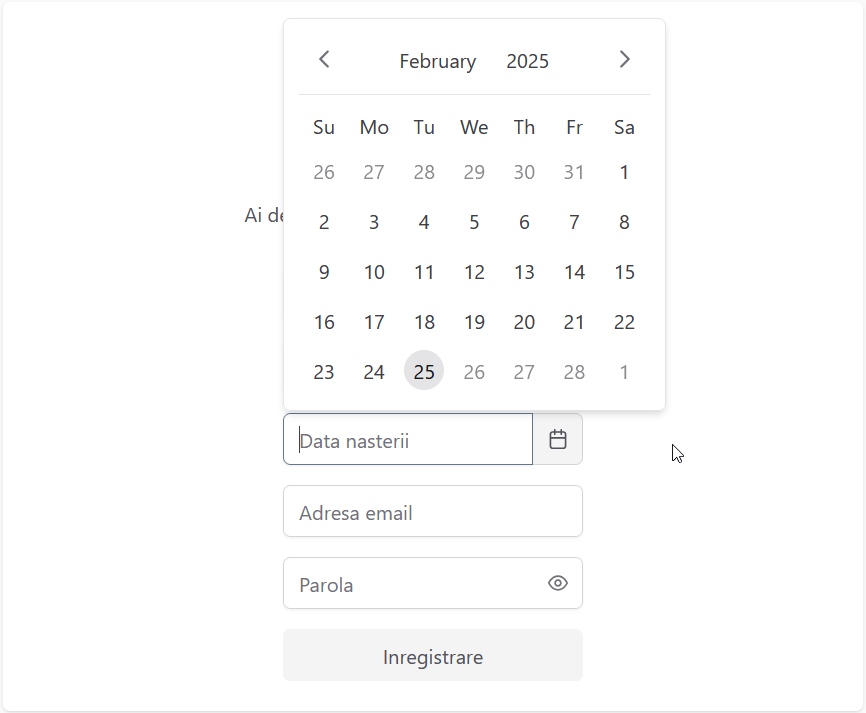
\includegraphics[width=\textwidth,height=0.8\textheight,keepaspectratio]{DatePicker.png}
  \caption{PrimeVue DatePicker component}\label{fig:datepicker}
\end{figure}

\FloatBarrier{}

As previously mentioned in~\ref{sec:techstack}, Vue also comes with other in-built tools that help create a well-working frontend. One of these tools is Vue Router, which was used to create the routes for the frontend. The student created a simple router that would allow the user to navigate between different pages. A navigation guard was used to protect the routes that required the user to be authenticated. An example of this can be seen below:

\begin{lstlisting}[caption=Vue Router Navigation Guard]
router.beforeEach(async (to) => {
  const authStore = useAuthStore()

  if (to.meta.requiresAuth) {
    await authStore.checkAuth() // Check if user is authenticated for protected routes
    if (!authStore.isAuthenticated) {
      return { name: 'Login' } // Redirect to login if not authenticated
    }
  } 
  // More code to handle other cases
})
export default router
\end{lstlisting}

Similarly, Pinia store was used to manage the authentication state of the user in the frontend. The store was then used by elements like the Navigation Guard to check if the user was authenticated before allowing them to access certain routes. An example of the store can be seen below:

\begin{lstlisting}[caption=Pinia Store for Authentication]
export const useAuthStore = defineStore('auth', () => {
  const isAuthenticated = ref(false)
  const user = ref(null)

  async function checkAuth() { // check if user is authenticated
    try {
      const response = await api.get('/me') // return user object if user is authenticated
      isAuthenticated.value = true // user is authenticated
      user.value = response.data.user
    }
    // More code to handle errors and no authentication
  }
  return { isAuthenticated, user, checkAuth }})
\end{lstlisting}

\subsection{Challenges}

\subsubsection{Lack of experience}

One of the biggest challenges encountered in this sprint was the lack of experience using some of the frameworks and libraries used in the project. As such, this sprint's progress moved slower due to the learning curve that needed to be overcome first by reading the documentation and finding any guides/help online.

\subsubsection{System-related decisions}

Another challenge was making decisions regarding different sections of the system, such as authentication, hashing algorithms, and others. Additional time was spent researching the best practices for each respective functionality \- analysing their advantages, disadvantages and ways to implement them in the current system.

\subsection{Requirements completed}

As this was the first sprint, the main focus was on setting up the groundwork for the project. The main requirements completed in this sprint were:

\begin{itemize}
    \item The system must provide a secure login mechanism for patients by using a combination of login and password.
    \item The database must store the user credentials in a secure manner.
    \item The system must be accessible on all modern desktop and mobile-based browsers.
    \item The system must allow patients to add their own personal information, such as name or date of birth.
    % TODO: Add more requirements
\end{itemize}

\section{Sprint \#2}

The second sprint of this project was focused on building some of the smaller elements of the system, such as the ability to add vaccines, allergies and medications. The decision to start with the smaller elements was made to allow the student to get a better understanding of how the frameworks used in the project worked and to get a better understanding of how to structure the project.

\subsection{Adding Vaccines, Allergies and Medications functionality}

The student started by creating the schemas for the Vaccines, Allergies and Medications tables in the database. These tables were created in a similar way to the User table, using SQLModel schemas. Afterwards, the student created the endpoints that would allow the user to add, update, delete and view the data in these tables.

On the frontend side, the system used Vue's main strengths to enable a smooth developer and future user experience. Some of the strengths used were using Vue components to create reusable elemenets, such as a Vaccine Card that would be used to display the vaccines that the user had added. The card also used other Vue elements such as props and emits to pass data between parent and child elements and pass events, respectively. An example of the Vaccine Card can be seen below:

\clearpage

\begin{lstlisting}[language=HTML, caption=Vue Vaccine Card Component Example]
<Card class="w-full" :pt="cardStyles">
  <template #title>
    <span class="font-bold text-2xl">{{ name }}</span>
  </template>
  <template #subtitle>
    <div class="flex items-center justify-between">
      <div>
        <span class="font-bold">{{ provider }}</span>
        <span>{{ date_received }}</span> 
      </div>
      <div>
        <Button icon="pi pi-eye" class="p-button-rounded p-button-text"
          @click="emit('showFile', props.id)" v-if="hasCertificate"/>
        <Button icon="pi pi-ellipsis-h" class="p-button-rounded p-button-text"
          @click="toggle"/>
        <Menu ref="menu" :model="items" :popup="true" />
      </div>
    </div>
  </template>
</Card>  
\end{lstlisting}

The VaccineCard component can then be easily used in the main view:

\begin{lstlisting}[language=HTML, caption=Using VaccineCard Component]
<VaccineCard
  v-for="vaccine in vaccines"
  :key="vaccine.id" 
  v-bind="vaccine"
  :has-certificate="!!vaccine.certificate"
  @delete="deleteVaccine"
  @open-edit="openEditDialog"
  @show-file="showCertificate"
/>
\end{lstlisting}

\begin{figure}[htbp]
  \centering
  
\includegraphics[width=\textwidth,height=0.7\textheight,keepaspectratio]{VaccineCard.png}
  \caption{Vue Vaccine Card component}\label{fig:vaccinecard}
\end{figure}

\FloatBarrier{}

This format was used across the system to easily create reusable components that could be used in multiple places, making the system more modular and easier to maintain.

To make sure the data displayed in the frontend was always up to date, the frontend used Vue's reactivity system. This allowed the data to be automatically updated whenever any change was made to the data in the backend or frontend. Examples of the reactivity system in use can be seen below, with functions that add and delete vaccines from the frontend when called:


\begin{lstlisting}[language=HTML, caption=Vue Reactivity System]
// Will add a vaccine to the vaccines array, which will automatically 
// create a new VaccineCard element
const addVaccine = (vaccine) => {
  vaccines.value.push(vaccine)
}

// Will remove a vaccine from the vaccines array, which will 
// automatically remove the VaccineCard element
const deleteVaccine = (id) => {
  vaccines.value = vaccines.value.filter((vaccine) => vaccine.id !== id)
}
\end{lstlisting}

\subsection{File Uploads}

Another major feature that was implemented in the 2nd sprint was the ability to upload files. At the time of implementation, the feature was only to be used for uploading vaccine certificates, however it could be easily extended to other parts of the system, such as uploading health records or lab results.

To allow a proper upload of files, a new table was created in the database, called FileUpload. This table contained the file metadata, such as its name, size, type, path and others. Similarly, a new table for Allergy Severity was created to ensure consistency in the user uploads and to allow for easy filtering and searching of the data.

The updated ERD diagram with the new tables can be seen below in figure~\ref{fig:erd_s2}:

\noindent\begin{minipage}{\textwidth}
  \begin{center}
      \rotatebox[origin=c]{270}{
          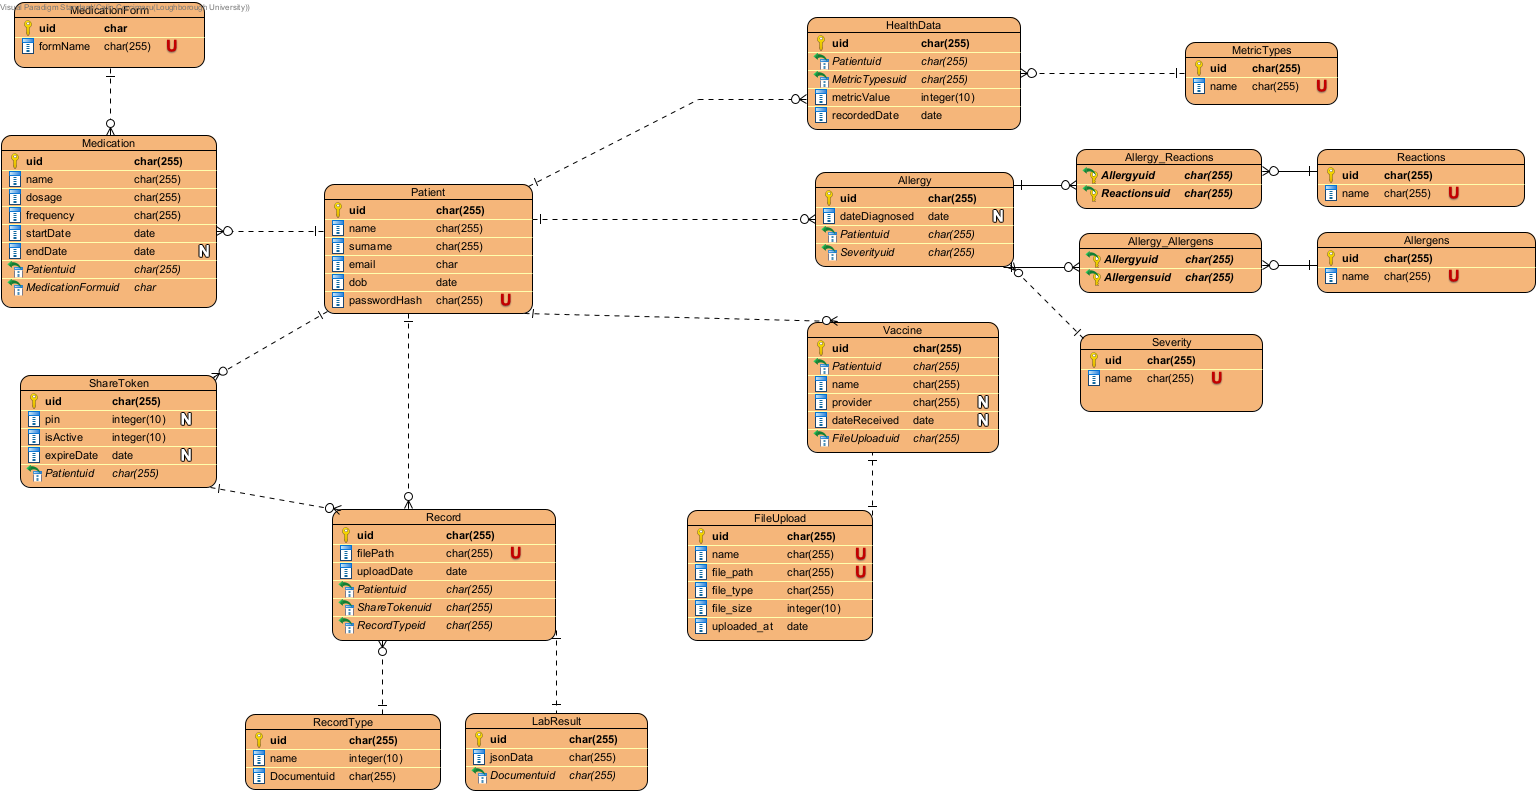
\includegraphics[width=0.95\textheight,keepaspectratio]{ERD_updatedS2.png}
      }
      \captionof{figure}{Updated Entity Relationship Diagram \- Sprint \# 2}\label{fig:erd_s2}
  \end{center}
\end{minipage}

To add more security to the system, the files were further encrypted before being stored in the database. AES was chosen as the encryption algorithm. Based on the articles analysed, it was consistently found to have the best balance between security and performance among other symmetric and asymmetric encryption algorithms \parencite{crypt1,crypt2,crypt3}. The choice to go with a symmetric algorithm was made due to its simplicity, as the key could be stored on the server-side in an environment variable, allowing the encryption and decryption of the files to be done on the server-side. This also allowed to avoid the issue of users losing access to their files if they lost their private encryption key, in the case of asymmetric encryption.

The encryption was done using the Fernet symmetric encryption algorithm from the cryptography library. Fernet uses AES-128 to encrypt the files. The key used to encrypt the files was stored in the environment variables and was generated when the system was started. In the interest of time, no rotation system for the key was implemented, however this would be a good feature to add in the future. 

The file upload process can be seen in figure~\ref{fig:fileuploadview} below. The file upload process was done in two steps. The first step was to upload the file to the server by using multipart form data. The next step would have the file be validated by checking its file type and size, then encrypted and stored in the file system and database. To access the files, the system used a new endpoint that would allow the user to download the file. The endpoint would take the file ID as a parameter and would stream the file to the user.

\begin{figure}[htbp]
  \centering
  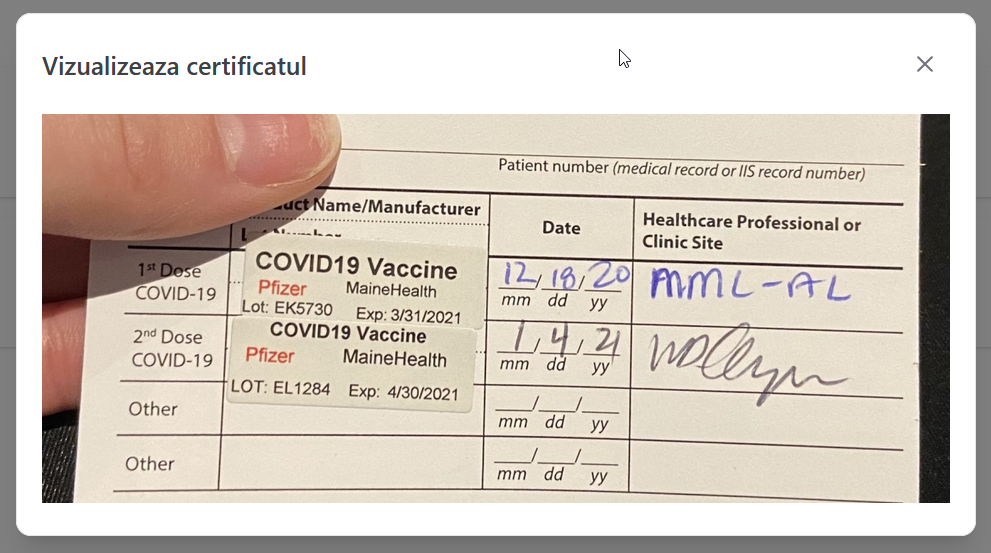
\includegraphics[width=\textwidth,height=0.7\textheight,keepaspectratio]{VaccineCertificate.png}
  \caption{Uploaded Vaccine Certificate}\label{fig:vaccinecertificate}
\end{figure}

\FloatBarrier{}

\begin{figure}[ht]
  \centering
  \subfloat[File Upload Sequence Diagram]{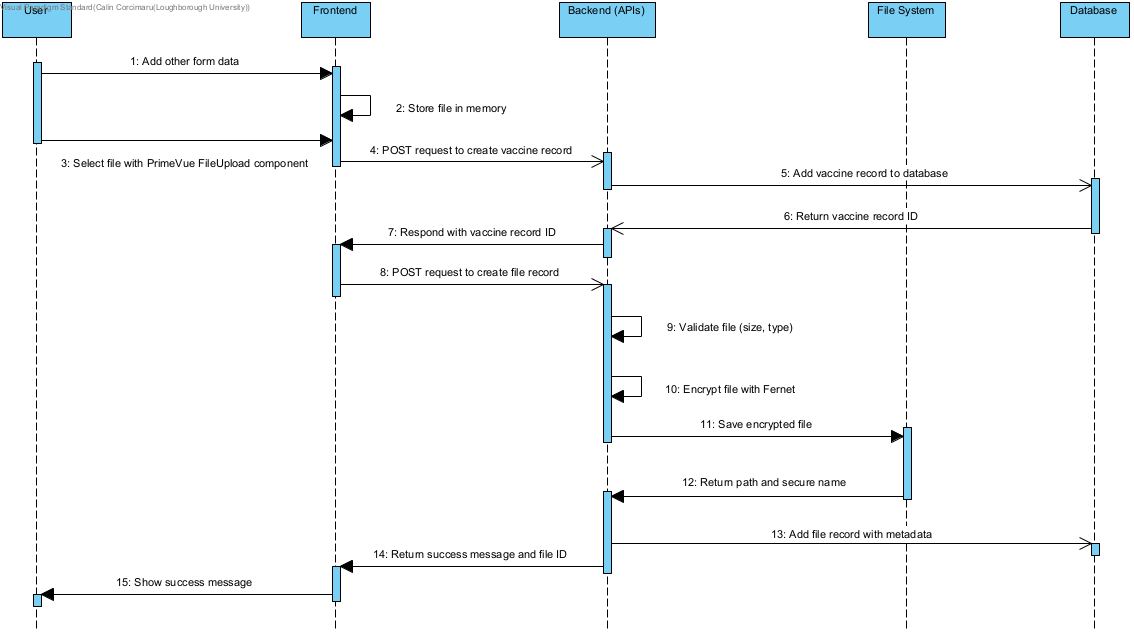
\includegraphics[width=\textwidth]{Sequence_FileUpload.png}\label{fig:seqfileupload}} 
  \\
  \subfloat[File View Sequence Diagram]{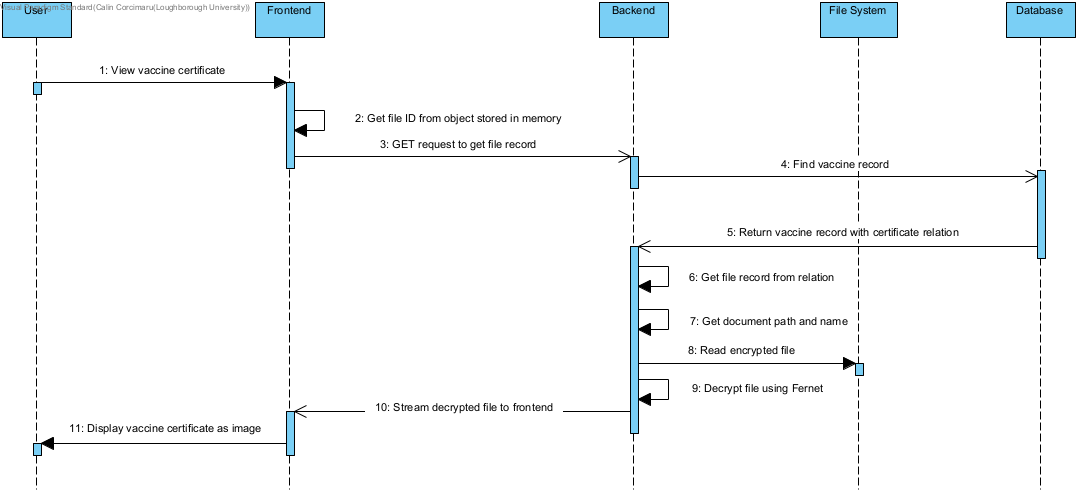
\includegraphics[width=\textwidth]{Sequence_FileView.png}\label{fig:seqfileview}} 
  \caption{Sequence Diagrams for File Upload and File View}\label{fig:fileuploadview}
\end{figure}

\FloatBarrier{}

The endpoint can be seen below:

\begin{lstlisting}[language=Python, caption=File Download Endpoint]
# Get a file by ID
@app.get("/files/{record_type}/{record_id}")
async def get_file(
  record_type: str,
  record_id: uuid.UUID,
  user_id: User = Depends(validate_session),
  session: Session = Depends(get_session)    
):    
  # Code to get the file record from the database
  
  async def get_data_from_file():
    with open(file_record.file_path, "rb") as f:
      encrypted_content = f.read()
      
    decrypted_content = decrypt_file(encrypted_content)

    yield decrypted_content
    
  return StreamingResponse(
    content=get_data_from_file(),
    media_type=file_record.file_type,
    status_code=status.HTTP_200_OK,
    headers={"Content-Disposition": f"inline; filename={file_record.name}"}
  )
\end{lstlisting}

Finally, the frontend was made with both mobile and desktop browsers in mind. This was achieved by using PrimeVue components and styling them with TailwindCSS. The system was also made to be responsive, so that it would look good on any screen size. Examples of the allergies page on both desktop and mobile can be seen below:

\begin{figure}[ht]
  \centering
  \subfloat[Desktop version]{%
      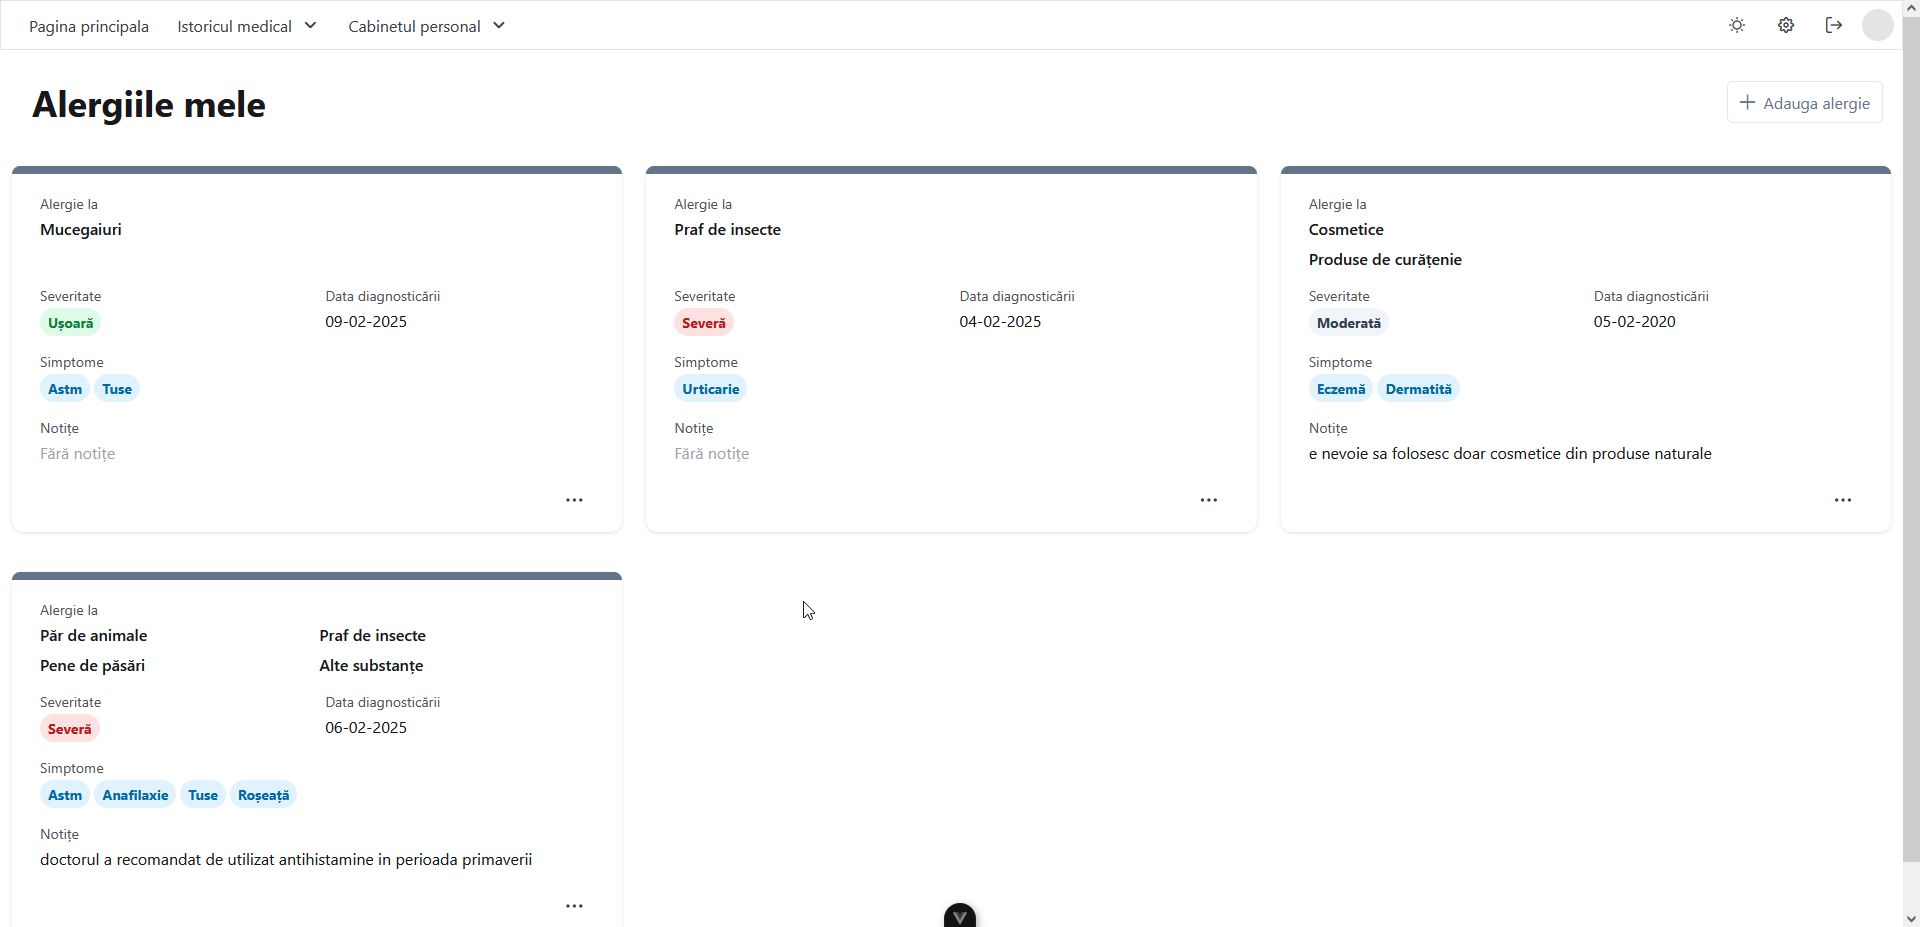
\includegraphics[width=\textwidth]{Desktop_AllergyView.png}%
  }
  \\[\baselineskip]
  \subfloat[Mobile version]{%
      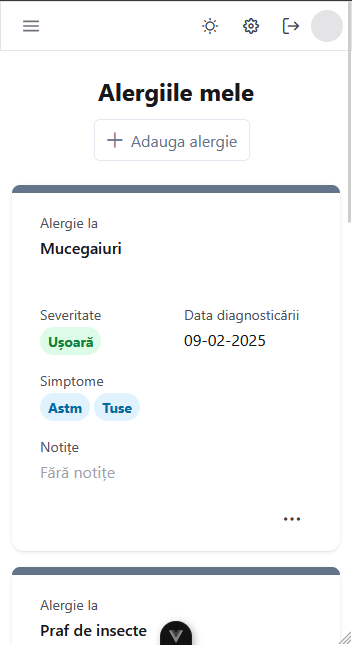
\includegraphics[width=0.4\textwidth]{Mobile_AllergyView.png}%
  }
  \caption{Desktop and Mobile version of the Allergies page}\label{fig:allergiespage}
\end{figure}

\FloatBarrier{}

\subsection{Challenges}

\subsubsection{Introducing new functionality}

In this sprint, the main challenge was introducing the new features/functionality in the system, while ensuring they worked properly together with both the existing frontend and backend. For some features, there was a need to revise and change some of the existing code, such as the API endpoints and even the database schemas to accommodate the newly implemented changes. This added some additional complexity, as it was crucial to ensure the changes did not break any of the existing functionality, while allowing the new features to work as intended.

\subsubsection{File Uploads}

Another challenge was understanding how some of the newly implemented features worked, such as the file upload system. It is important to note that the student had no previous experience implementing any file upload functionality, so extra time and work was dedicated to ensure the relevant documentation was studied and then implemented correctly.

\subsubsection{System complexity}

Finally, due to lack of time and poor initial planning because of the complexity of the system, some of the features intended for this sprint had to be moved to the next one. Some examples include the health data section and also the main dashboard parts for vaccines, allergies, medications and health data. 

These changes and challenges show that undertaking a more agile approach to the project was beneficial, as the project embraces change and allows for more flexibility in the development process.

\subsection{Requirements completed}

The main requirements completed in this sprint were:

\begin{itemize}
    \item The system must store the data in a secure manner, ensuring that only the patient and the doctor can access the data.
    \item The system must allow patients to upload their own medical records in a variety of formats (PDF, DOC, etc).
    \item The system should allow to upload files/documents for other types of records (vaccine certificates, etc).
    \item The system must allow the patient to add their own allergies.
    \item The system must allow the patient to add their own vaccinations.
    \item The system must allow patients to enter their current medication including details such as the name of the drug, dosage, frequency and start/end date.
    \item The system must allow patients to add new medication to their list.
\end{itemize}

\section{Sprint \#3}

The third sprint of the project was focused on building the main dashboard view of the system, which would display an overview of the most recent records added, such as vaccines, allergies, medications, etc. Additionally, another aim for this sprint was to complete the vital signs feature of the system, which would allow patients to add information such as weight or blood pressure in both a tabular and graphical format. 

All these features were part of the initial requirements discussed with the stakeholders, and were chosen to be completed in this sprint as their technical implementation was similar to more complex features that would be implemented in the future, which would help build additional proficiency in the frameworks and libraries used in the project.

However, besides the above-mentioned features, additional work had to be done on how the information is displayed in the frontend. This was a change requested by one of the stakeholders, based on their feedback after the sprint 2 features were presented to them. As such, additional time had to be spent on reworking the frontend to better display the information in a more user-friendly and consistent way. 

\subsection{Updated frontend}

One of the main feedback received from the stakeholders was the inconsistency in how the information was displayed for some of the sections in the system, such as the vaccines, allergies and medications. This was due to the different amount of information each record contained: vaccines contained the least amount of information, followed by allergies and medications. As such, some records were stored in a grid view, while others were stored in a list view. Also, some cards had different ways of displaying the information, such as using tags or colored lines, etc. 

The decision was made to keep things simple, by removing unnecessary colors and ensuring that there would be consistency in how the cards were displayed \- either by having only one type of view (grid/list) or offering both for the user to choose from. Tags were kept as they allowed for an easy way to display the information in a more readable way.

Thankfully, PrimeVue offered an easy way to re-work the frontend thanks to its Data View component \- a flexible component that could be used to display data in a grid or list view. The component also offered a way to customize the data displayed, such as adding tags, icons, etc. 

An example of the updated allergies page can be seen below in figure~\ref{fig:allergiespagev2}. The page now offers both a grid and list view, which can be toggled by the user. The page also offers a more consistent way of displaying the information, with each card containing the same information, but displayed in a different way depending on the view chosen.

\begin{figure}[ht]
  \centering
  \subfloat[Desktop version]{%
      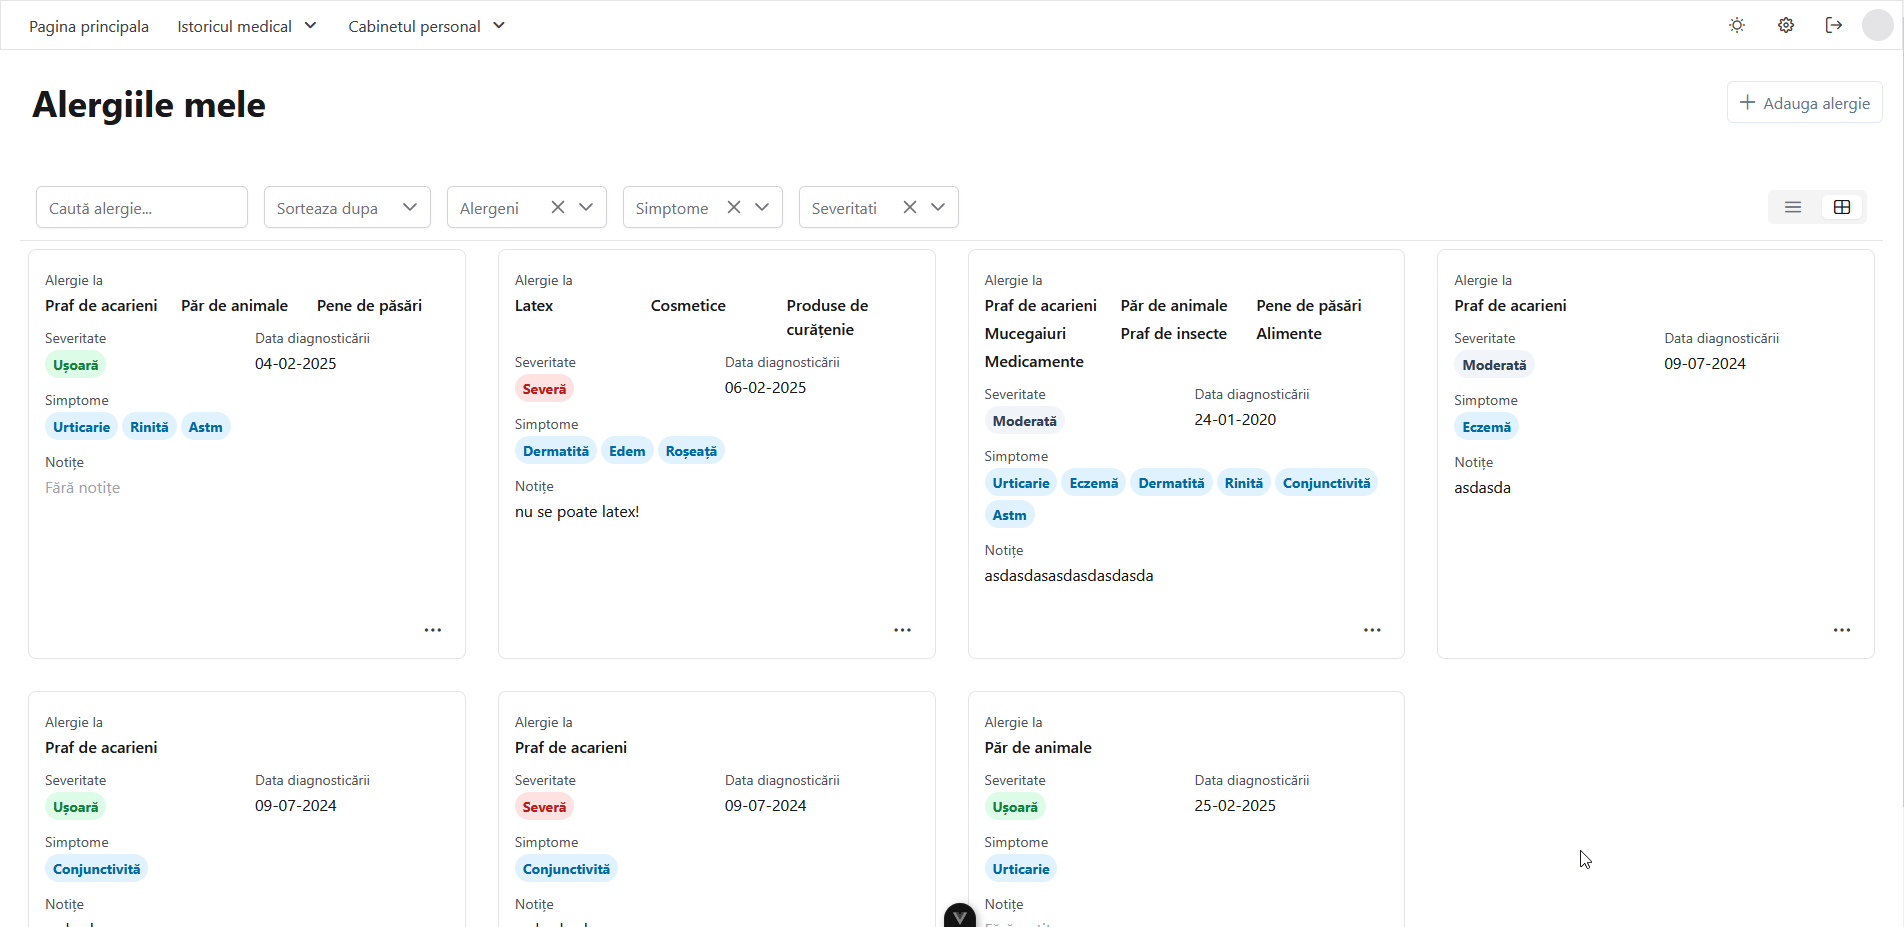
\includegraphics[width=\textwidth]{Desktop_AllergyView_v2.png}%
  }
  \\[\baselineskip]
  \subfloat[Mobile version]{%
      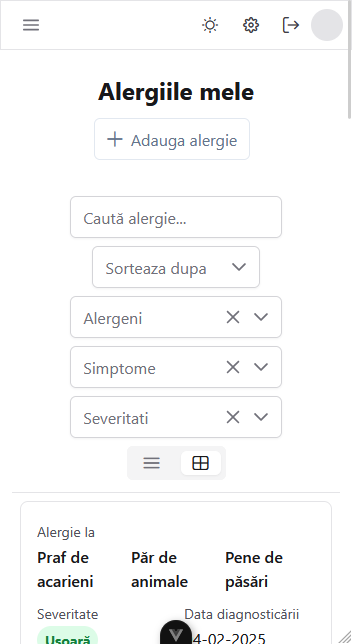
\includegraphics[width=0.4\textwidth]{Mobile_AllergyView_v2.png}%
  }
  \caption{Desktop and Mobile version of the Allergies page \- 2nd version}\label{fig:allergiespagev2}
\end{figure}

\FloatBarrier{}

\subsection{Filtering and sorting}

Another feedback provided by the stakeholders was the ability to filter and sort the information displayed in the system. This was especially important for the medications, where a patient could have multiple medications and would want to quickly find a specific one. Suggestions for this feature was to mainly add a search bar that would allow the user to find a specific record, however the stakeholders added that it would be nice to have some sorting/filtering options like sorting by date added or filtering based on type of medication, allergy severity, etc.

Sorting and filtering was implemented in the frontend by using Vue's reactivity system, powered by the ref and computed functions. The ref function was used to create reactive variables that would be updated whenever the data changed. The computed function was used to create computed properties that would be updated whenever the reactive variables changed. As such the sort query could be stored within a reactive variable, while the computed function would change the data displayed based on the sort query.

An example of the sorting and filtering functionality can be seen below:

\begin{lstlisting}[language=HTML, caption=Medication Sorting and Filtering]
  const filteredMedicine = computed(() => {
    return props.medications.filter((medication) => {
      return medication.name.toLowerCase().includes(searchQuery.value.toLowerCase())
    })
  })
\end{lstlisting}

\begin{lstlisting}[language=HTML, caption=Allergies Sorting and Filtering]
  const filteredAllergies = computed(() => {
  
  if (selectedAllergens.value.length > 0) {
    return props.allergies.filter((allergy) =>
      allergy.allergens.some((allergen) => selectedAllergens.value.includes(allergen))
    )
  }

  if (selectedReactions.value.length > 0) {
    return props.allergies.filter((allergy) =>
      allergy.reactions.some((reaction) => selectedReactions.value.includes(reaction))
    )
  }

  if (selectedSeverities.value.length > 0) {
    return props.allergies.filter((allergy) =>
      selectedSeverities.value.includes(allergy.severity)
    )
  }  

  return props.allergies.filter((allergy) =>
    allergy.allergens.some((allergen) =>
      allergen.toLowerCase().includes(searchQuery.value.toLowerCase())
    )
  )
})  
\end{lstlisting}

\subsection{Vital Signs}

Coming back to the sprint's focus, one of the main features intended to be implemented was the vital signs feature. This feature would allow the patient to add their own vital signs, such as weight, height, blood pressure, etc. The data would be displayed in both a tabular and graphical format, allowing the patient to see their progress over time.

When discussing this requirement with the stakeholders, a suggestion was given to display the most recent/current health data point added in a separate card, so that a patient could view their most recently added information easily. Additionally, a suggestion was given to display an arrow/icon near the value of the vital data point to show whether the value was above or below versus the previous value.

To display the data in a tabular and graphical view, the system uses PrimeVue's Data Table component and Chart.js library respectively. Examples of how the Vitals page looks can be seen below in figure~\ref{fig:vitalspage} and~\ref{fig:vitalspagegraph}.

\begin{figure}[ht]
  \centering
  \subfloat[Desktop version]{%
      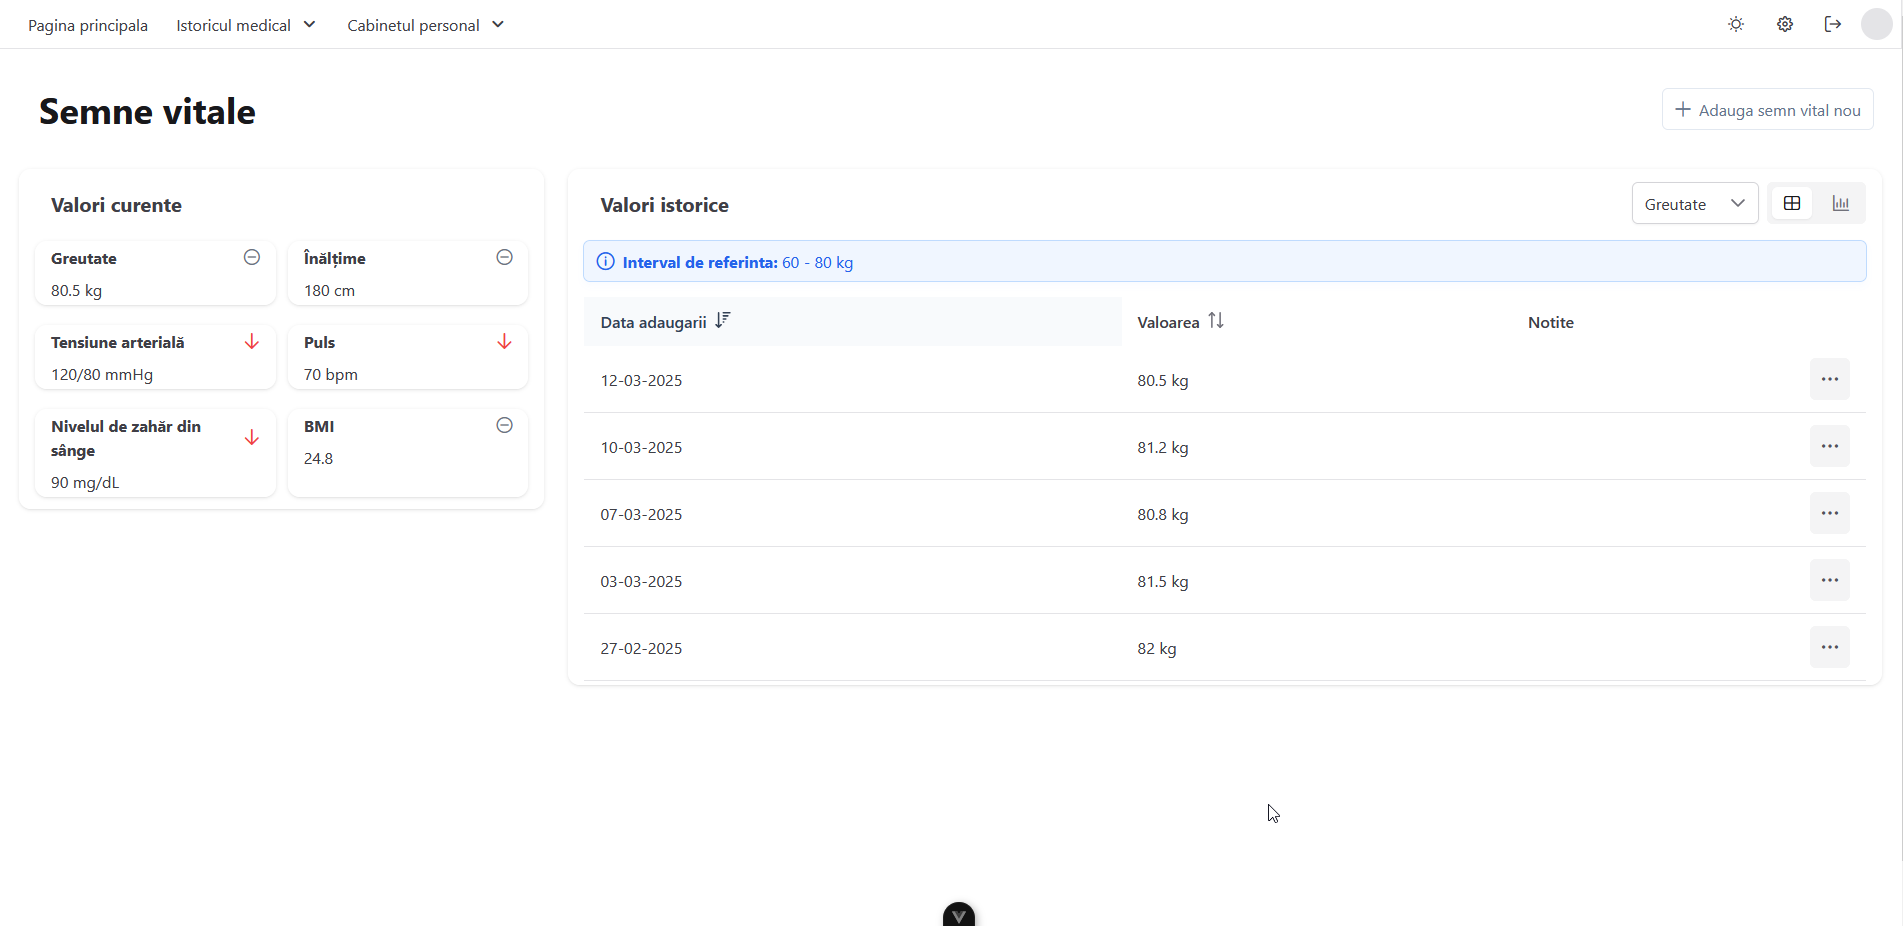
\includegraphics[width=\textwidth]{Desktop_VitalsView.png}%
  }
  \\[\baselineskip]
  \subfloat[Mobile version]{%
      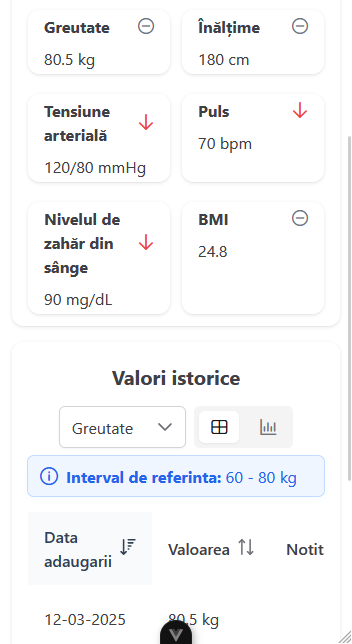
\includegraphics[width=0.4\textwidth]{Mobile_VitalsView.png}%
  }
  \caption{Desktop and Mobile version of the Vitals page}\label{fig:vitalspage}
\end{figure}

\FloatBarrier{}

\begin{figure}[ht]
  \centering
  \subfloat[Desktop version]{%
      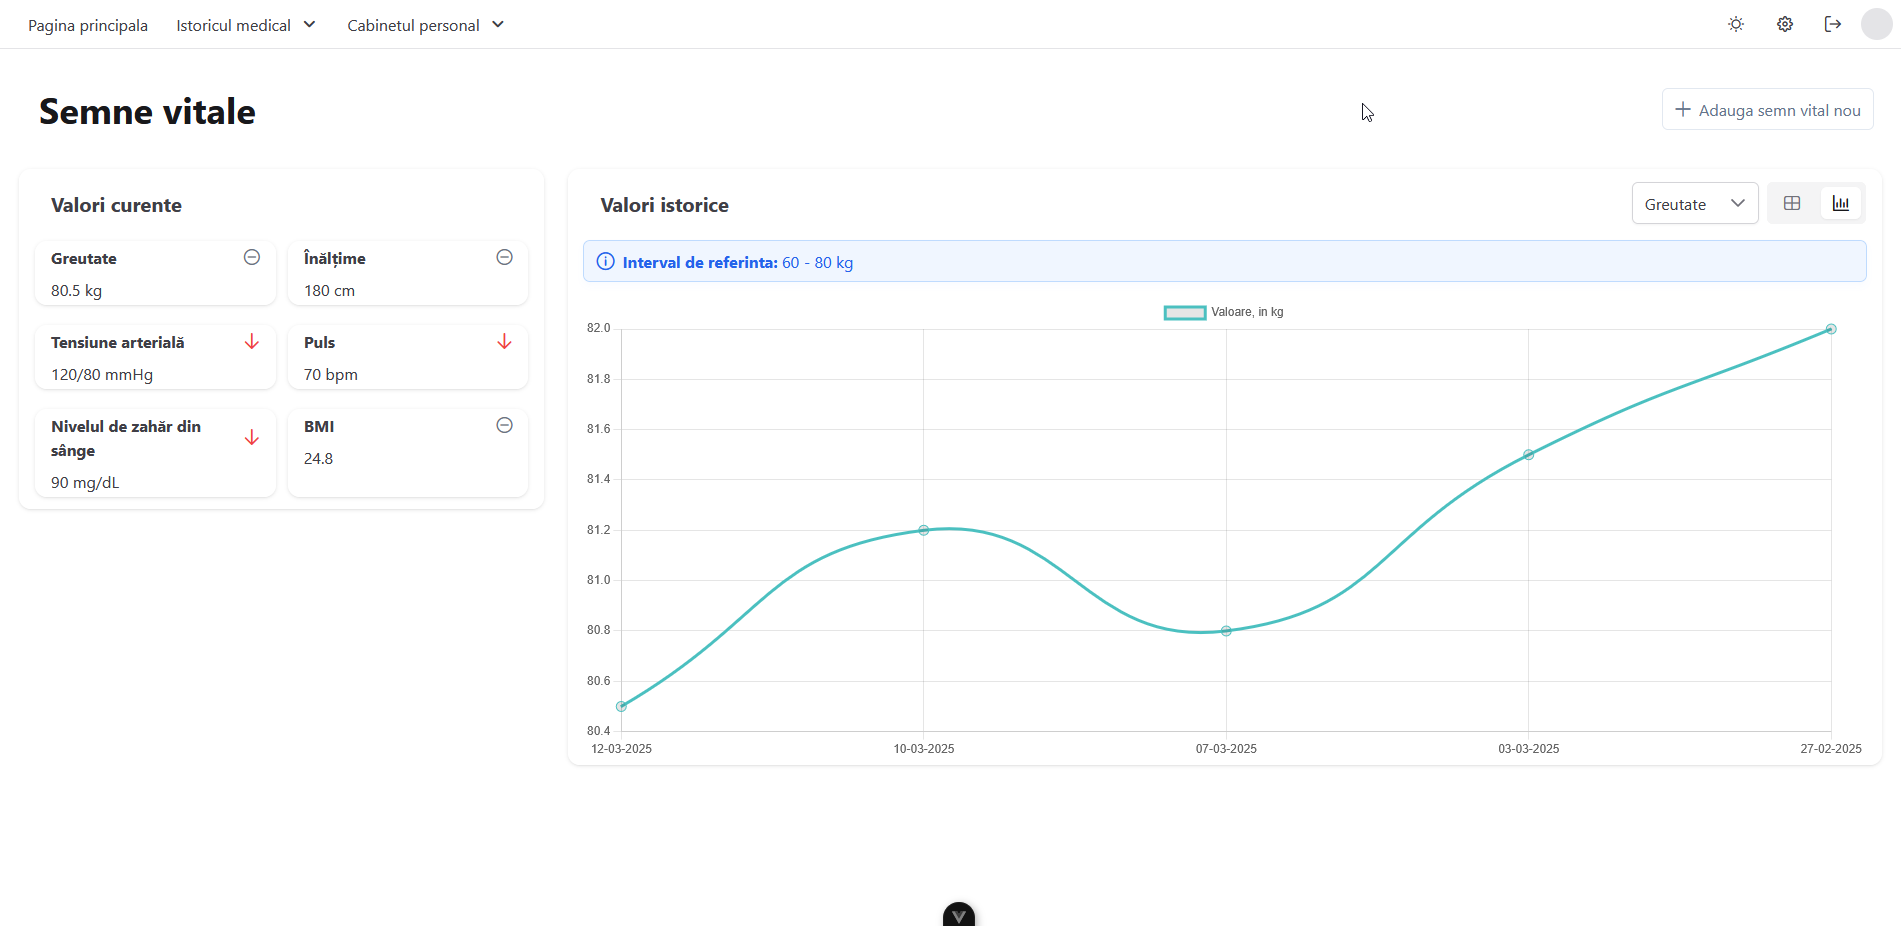
\includegraphics[width=\textwidth]{Desktop_VitalsView_Graph.png}%
  }
  \\[\baselineskip]
  \subfloat[Mobile version]{%
      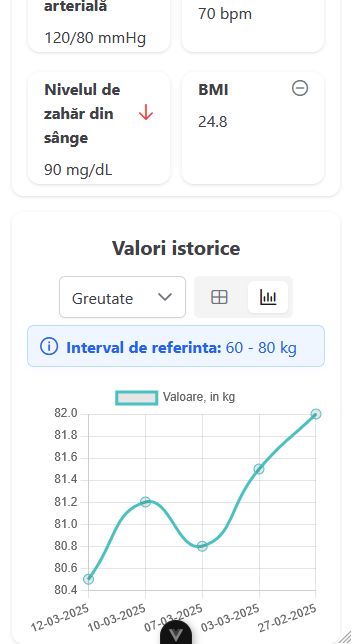
\includegraphics[width=0.4\textwidth]{Mobile_VitalsView_Graph.png}%
  }
  \caption{Desktop and Mobile version of the Vitals page, with Graph}\label{fig:vitalspagegraph}
\end{figure}

\FloatBarrier{}

\subsection{Dashboard}

Finally, the other main feature added was the ability for patients to have a dashboard-type view of the most recent records/information added to their account. The decision was made to display only the 5 most recent records for each section, encouraging the user to go to their respective page if they wanted to see more or see the records in more detail. The structure of each record was kept similar as to how they were displayed in their own pages to maintain consistency, so things like tags were still used to ensure a patient would know what they are looking for at the dashboard.

Similar to the vital signs feature, the Data Table view component from PrimeVue was used to create the individual tables for each of the section, making the development of the dashboard feature simple and easy. Each section was an individual Vue component, which was then imported into the dashboard main Vue view. An example of a section code can be seen below:

\begin{lstlisting}[language=HTML, caption=Vital Signs Dashboard Section Component]
<template>
  <Card :pt="cardStyles" class="h-full">
    <template #title>
      <h2 class="text-xl font-bold p-4">Semne vitale recent adaugate</h2>
    </template>
    <template #content>
      <DataTable :value="props.vitals" removableSort>
        <Column field="name" header="Numele" sortable> </Column>
        <Column field="value" header="Valoarea" sortable>
          <template #body="slotProps">
            <span v-if="slotProps.data.value">
              {{ slotProps.data.value }} {{ slotProps.data.unit }}
            </span>
            <span v-else>
              {{ slotProps.data.value_systolic }}/{{ slotProps.data.value_diastolic }}
              {{ slotProps.data.unit }}
            </span>
          </template>
        </Column>
        <Column field="date_recorded" header="Data adaugarii" sortable>
          <template #body="slotProps">
            <span> {{ slotProps.data.original_date_recorded }} </span>
          </template>
        </Column>
      </DataTable>
    </template>
    <template #footer>
      <RouterLink to="/vitale" class="p-button p-button-text">Vezi toate semnele vitale</RouterLink>
    </template>
  </Card>
</template>
\end{lstlisting}

Finally, the dashboard view can be seen below in figure~\ref{fig:dashboardpage}.

\begin{figure}[ht]
  \centering
  \subfloat[Desktop version]{%
      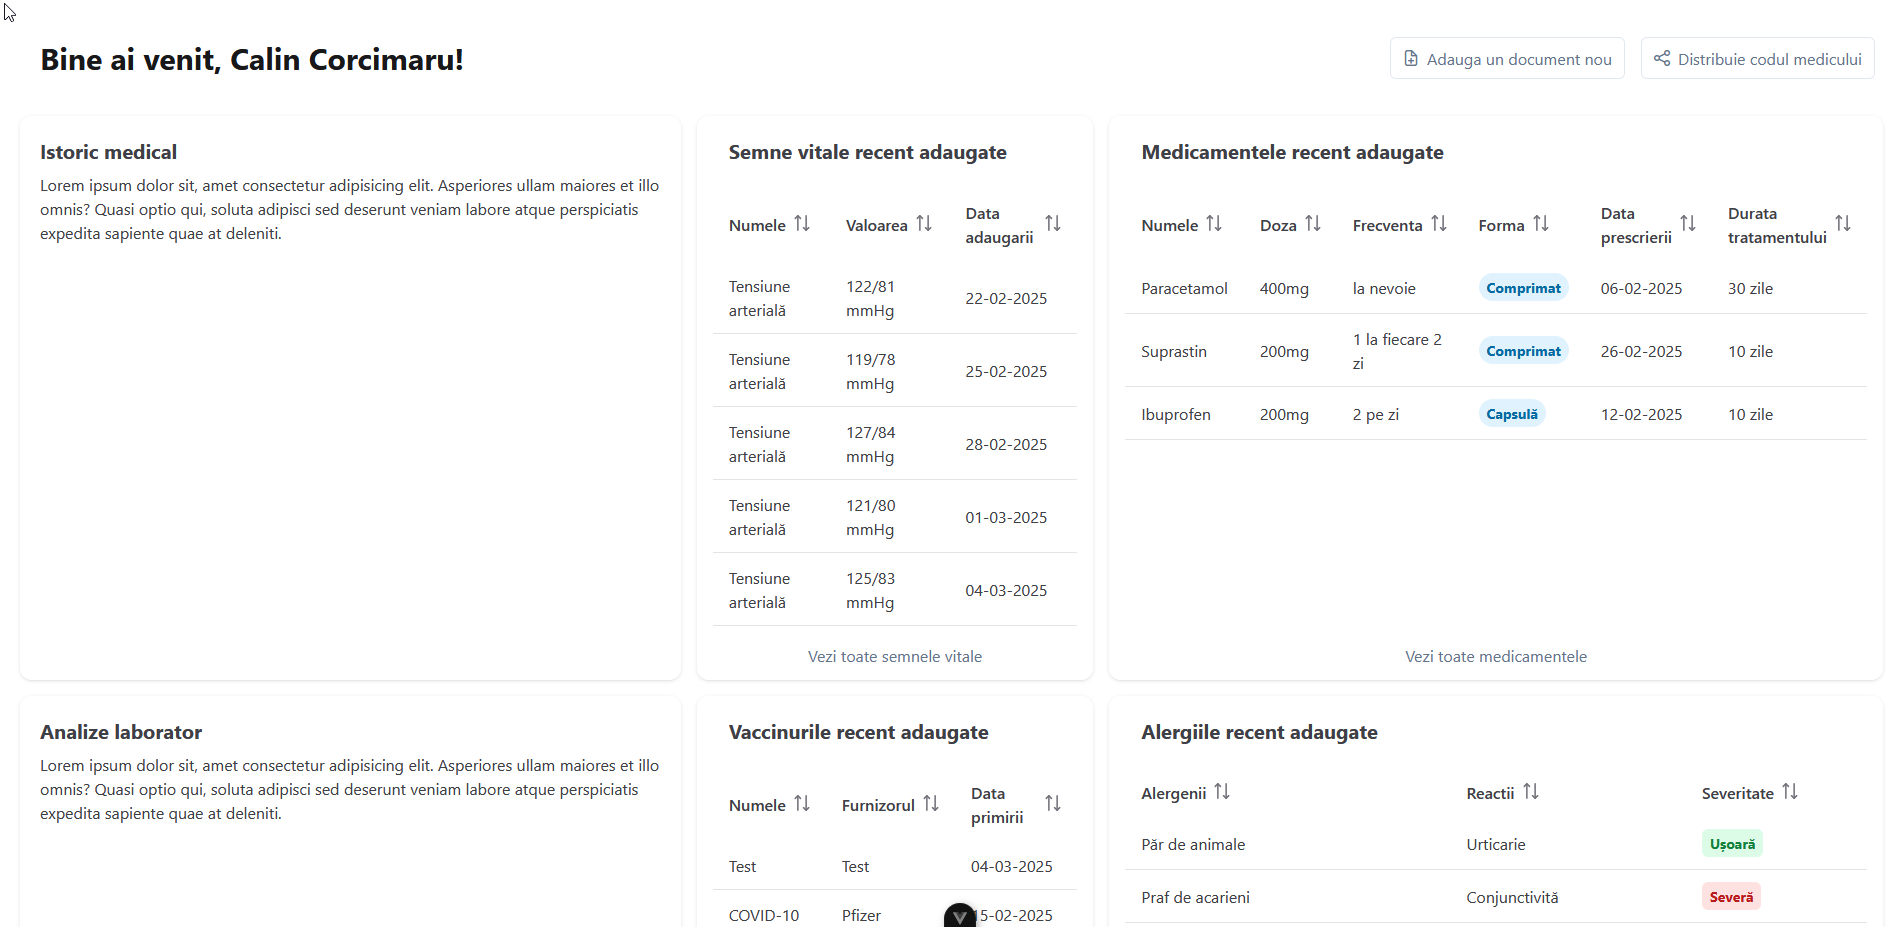
\includegraphics[width=\textwidth]{Desktop_DashboadView.png}%
  }
  \\[\baselineskip]
  \subfloat[Mobile version]{%
      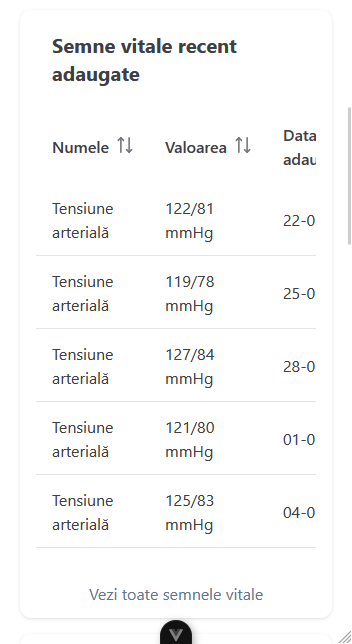
\includegraphics[width=0.4\textwidth]{Mobile_DashboardView.png}%
  }
  \caption{Desktop and Mobile version of the Dashboard page}\label{fig:dashboardpage}
\end{figure}

\FloatBarrier{}

\subsection{Backend changes}

While the focus of this sprint was mainly the frontend, there were some parts of the backend that needed to be changed to accommodate some of the implemented changes. 

One change made was the addition of a database table for the vital data points, which would contain the type name, such as Weight, the unit of measurement and a normal range, all of which was then used or displayed on the vitals page. Another change to the database was the addition of a new field, called date\_added to all of the tables/records in the system. This field was used mainly used to sort and determine the most recently added records to the system, which could be a different value to the other dates already used in the records' tables. An example could be found in vaccines: a vaccine could've been received years ago, but it could be added anytime to the system. As such, the record can have 2 different dates associated with it: the date the vaccine was actually received and the date it was added to the system. As such, the updated database schema can be found below:

\noindent\begin{minipage}{\textwidth}
  \begin{center}
      \rotatebox[origin=c]{270}{
          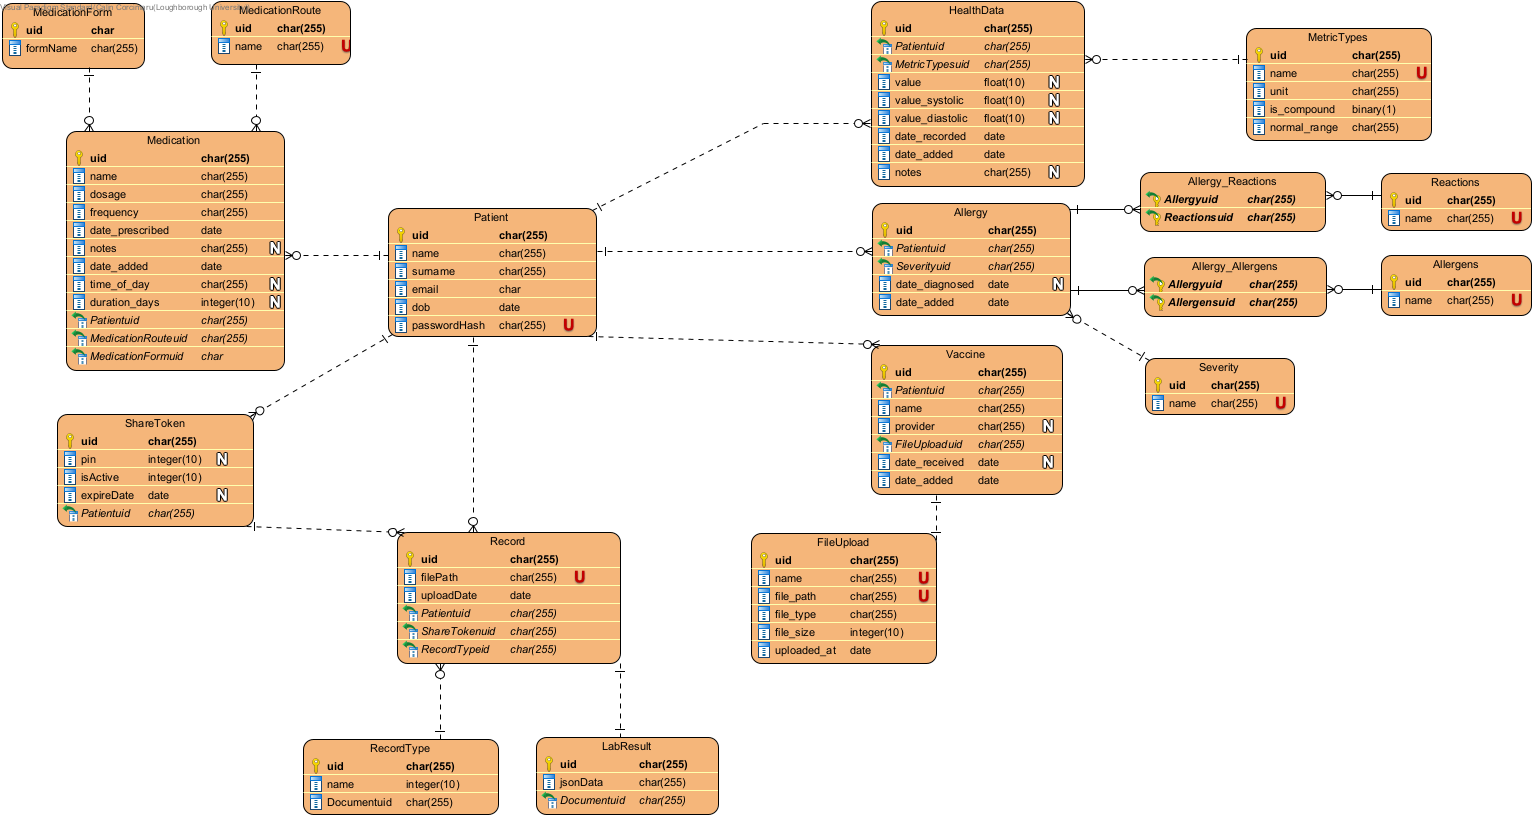
\includegraphics[width=0.95\textheight,keepaspectratio]{ERD_updatedS3.png}
      }
      \captionof{figure}{Updated Entity Relationship Diagram \- Sprint \#3}\label{fig:erd_s3}
  \end{center}
\end{minipage}

Other changes included multiple changes to the API endpoints, mainly relating to the vital signs data, due to the addition of the new table and its contents. Similarly, a new endpoint for the dashboard had to be created, which would use the newly added date\_added field to sort through the 5 most recent records in each category and send them back as the response. Below can be found the code that sorts and selects the 5 most recent records for each category:

\begin{lstlisting}[language=Python, caption=Dashboard Endpoint]
@app.get("/dashboard", response_model=UserDashboard)
async def get_dashboard(user_id: uuid.UUID = Depends(validate_session), session: Session = Depends(get_session)):
    user = session.get(User, user_id)
    
    if user_id != user.id:
        raise HTTPException(status_code=403, detail="You do not have permission to access this endpoint!")   
    
    newest_vaccines = session.exec(select(Vaccine).where(Vaccine.user_id == user_id).order_by(col(Vaccine.date_added).desc()).limit(5)).all()
    newest_allergies = session.exec(select(Allergy).where(Allergy.user_id == user_id).order_by(col(Allergy.date_added).desc()).limit(5)).all()
    newest_healthdata = session.exec(select(HealthData).where(HealthData.user_id == user_id).order_by(col(HealthData.date_added).desc()).limit(5)).all()
    newest_medications = session.exec(select(Medication).where(Medication.user_id == user_id).order_by(col(Medication.date_added).desc()).limit(5)).all()
    
    # Code that transforms each record into a response object...

    user_dashboard = UserDashboard(
        id = user.id,
        name = user.name,
        vaccines = vaccines_response,
        allergies = allergies_response,
        vitals = healthdata_response,
        medications = medications_response
    )
    
    return user_dashboard
\end{lstlisting}

\subsection{Challenges}

\subsubsection{Scope Creep}

One of the main challenges encountered in this sprint was the scope creep and the change in requirements. While an initial discussion was done with stakeholders and wireframes were created to have a shared understanding regarding how the system should look, further discussions brought up areas of improvement and change opportunities within the system. This led to additional work being done on both the frontend and backend to ensure the system was adhering to stakeholder expectations, and that it provides a pleasant user experience and enough functionality to be a viable solution for the market.

\subsubsection{Infrequent communication with stakeholders}

One of the main problems encountered in this sprint and the previous ones was the infrequent communication with stakeholders. This was caused by many factors, such as the busy schedules of both the student and the stakeholders, their other commitments such as studies or other work positions, but also the fact that all communication was done virtually, limiting the interaction to meetings or messages via communication apps. This infrequent communication led to situations where the student might have had to make decisions regarding the system design on their own, which could not have been liked by stakeholders, requiring changes or re-doing, adding additional work load on the student. 

As such, it was clear that for the upcoming sprints, a more constant communication between the student and stakeholders needed to be established to ensure that what was worked on was in line with the stakeholders' expectations.

\subsubsection{Lack of proper testing procedures}

Due to the complexity of the system and time pressure, barely any kind of automated testing was implemented. This lead to unexpected issues appearing in the course of development, which created additional work for the student, changing their focus from the sprint items to fixing the bugs, thus delaying the sprint completion. The student also doesn't have much experience creating tests for the frontend, which made the testing process even more difficult, leading to many of the testing to be done manually or skipped entirely. Due to the limited time remaining, it might be necessary to dedicate a part of the upcoming sprints to do some more thorough testing to ensure that the system as a whole does not have any critical bugs or issues that may affect its functionality.

\subsection{Requirements completed}

\begin{itemize}
    \item The system must have a dashboard view which displays an overview of the most recent information added to the system (latest lab tests, doctor consultations, vaccinations etc).
    \item The system should display the health records in both a list or grid view.
    \item The system should allow the patient to enter vitals information, such as height, weight, blood pressure, etc.
    \item When multiple vital entries are made, the system could display a historical graph of the patient's vitals.
    % TODO: Add more requirements
\end{itemize}

\section{Sprint \#4}

The fourth sprint of the project focused on adding the ability to add health records, such as lab tests, doctor consultations or imaging results. This was one of the main features requested by the stakeholders, as it would allow a patient to have all their medical history in one place, making it easier for them to view and share it with their doctors.

Additionally, at the end of sprint \#3, the stakeholders provided feedback regarding the features implemented in the previous sprint. Some of the feedback included:

\begin{itemize}
    \item The graph in the Vitals page should show the normal range for that specific vital type in graph.
    \item The Vitals signs page should have a date filtering functionality to choose a date range for the signs displayed in the graph or table.
    \item Weight and height should not have a normal range.
    \item Previously, the trend most recent vitals signs were compared with the 2nd most recent ones, which was not a good choice for comparison. The most recent vitals signs should be compared with the normal range for that specific vital type.
    \item On the main dashboard, the most recent vitals section should show the most recent values for one each type of vital signs, instead of the most recent 5 values for each type.
    \item On the main dashboard, only the allergies with moderate and severe allergies should be displayed.
\end{itemize}

\subsection{Health Records}

As mentioned in the introduction to this section, the main focus of this sprint was creating the functionality to add health records such as lab tests, doctor consultations or imaging results in the system. This was a crucial feature and a main requirement of the system, as it would allow patients to create their medical history in the system, upload the files associated with these records and then refer to them whenever needed or share them with doctors to allow them to have a more accurate patient history and thus offer better treatment.

The choice was made to display the record history in a tabular format, as that would allow to display the important information in a readable way, but also to sort the information based on different fields such as the date of the consultation or filter by fields such as doctor or institution name for easier search. PrimeVue has a DataTable component, which allowed the inclusion of all these features with little effort that are displayed in a user-friendly way. An example of the health records page can be seen below in figure~\ref{fig:healthrecordspage}.

\begin{figure}[ht]
  \centering
  \subfloat[Desktop version]{%
      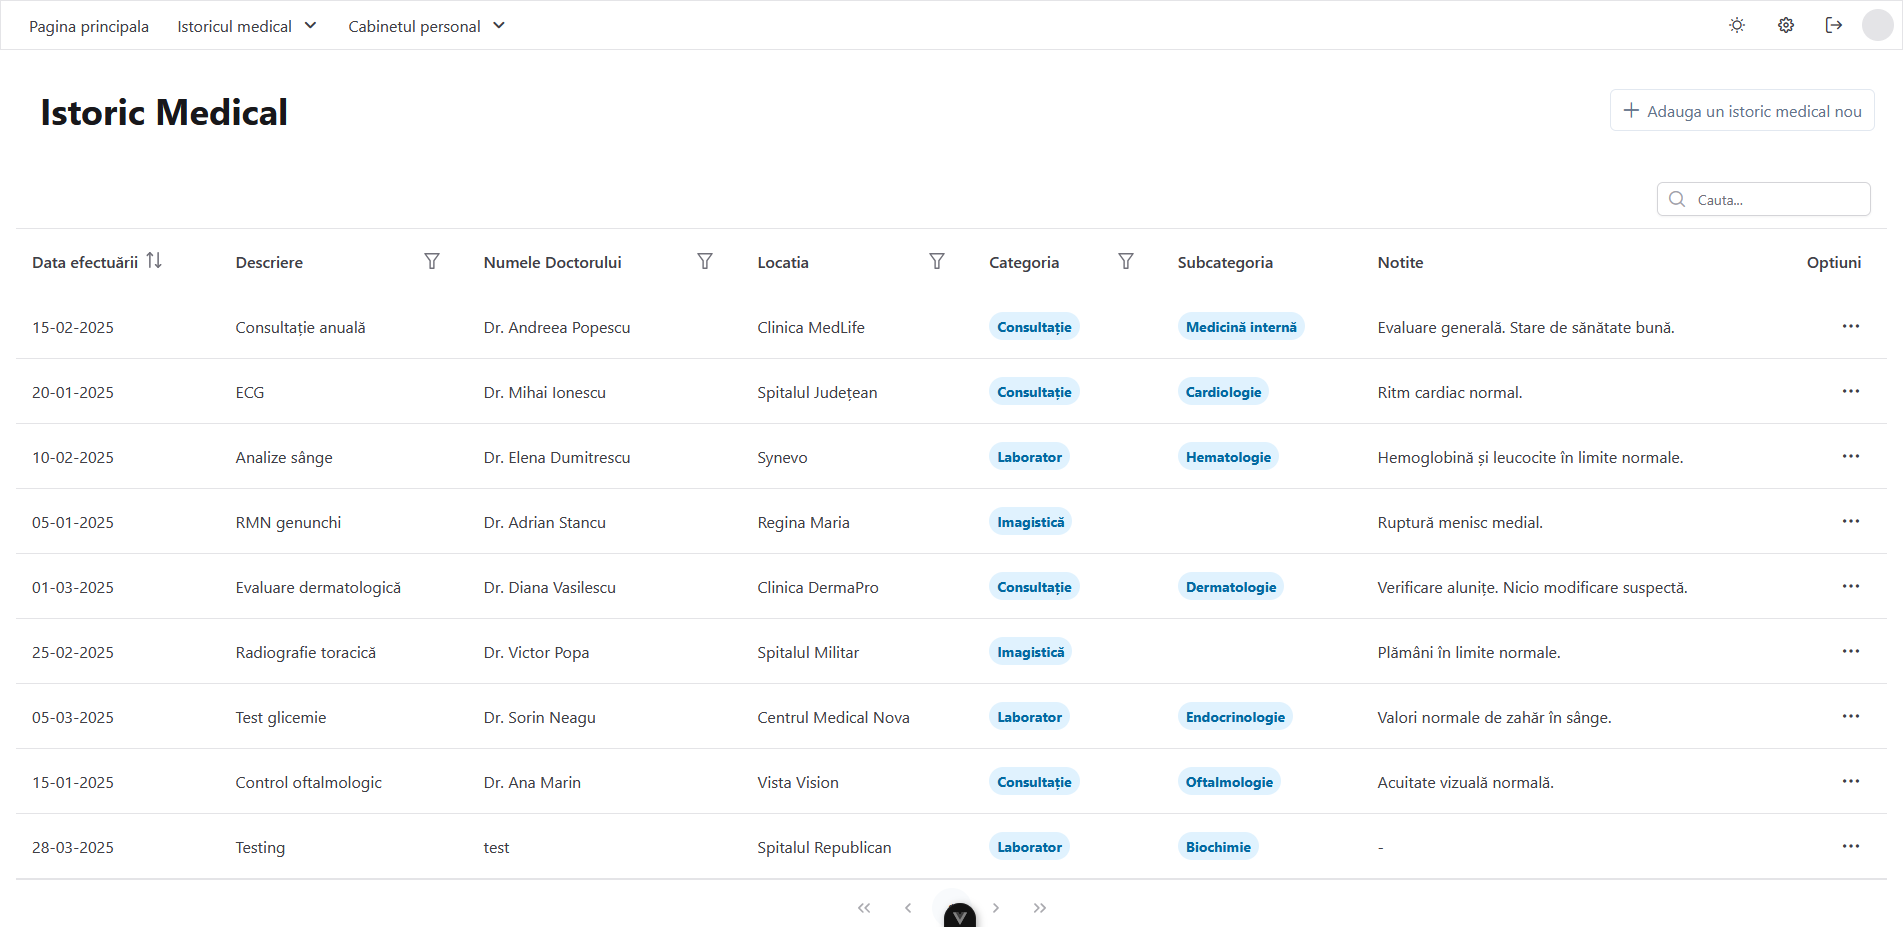
\includegraphics[width=\textwidth]{Desktop_HistoryView.png}%
  }
  \\[\baselineskip]
  \subfloat[Mobile version]{%
      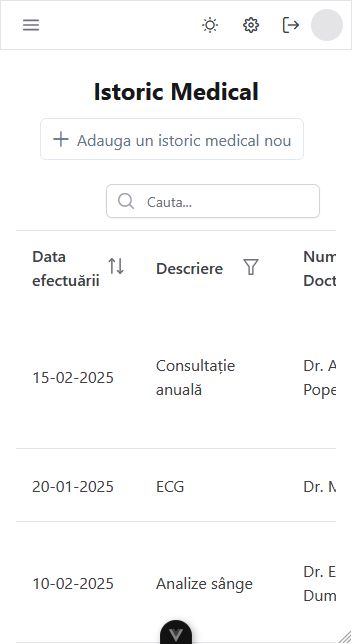
\includegraphics[width=0.4\textwidth]{Mobile_HistoryView.png}%
  }
  \caption{Desktop and Mobile version of the History page}\label{fig:healthrecordspage}
\end{figure}

\FloatBarrier{}

DataTable also comes with an in-built filtering option, which allowed to add a search bar for the whole table, but also search functions for specific fields. Example of the search bar can be seen in the screenshots above, and the filter menu can be seen below in figure~\ref{fig:filtermenu}. A code snippet of the filter function in a column can also be seen below.

\begin{figure}[htbp]
  \centering
  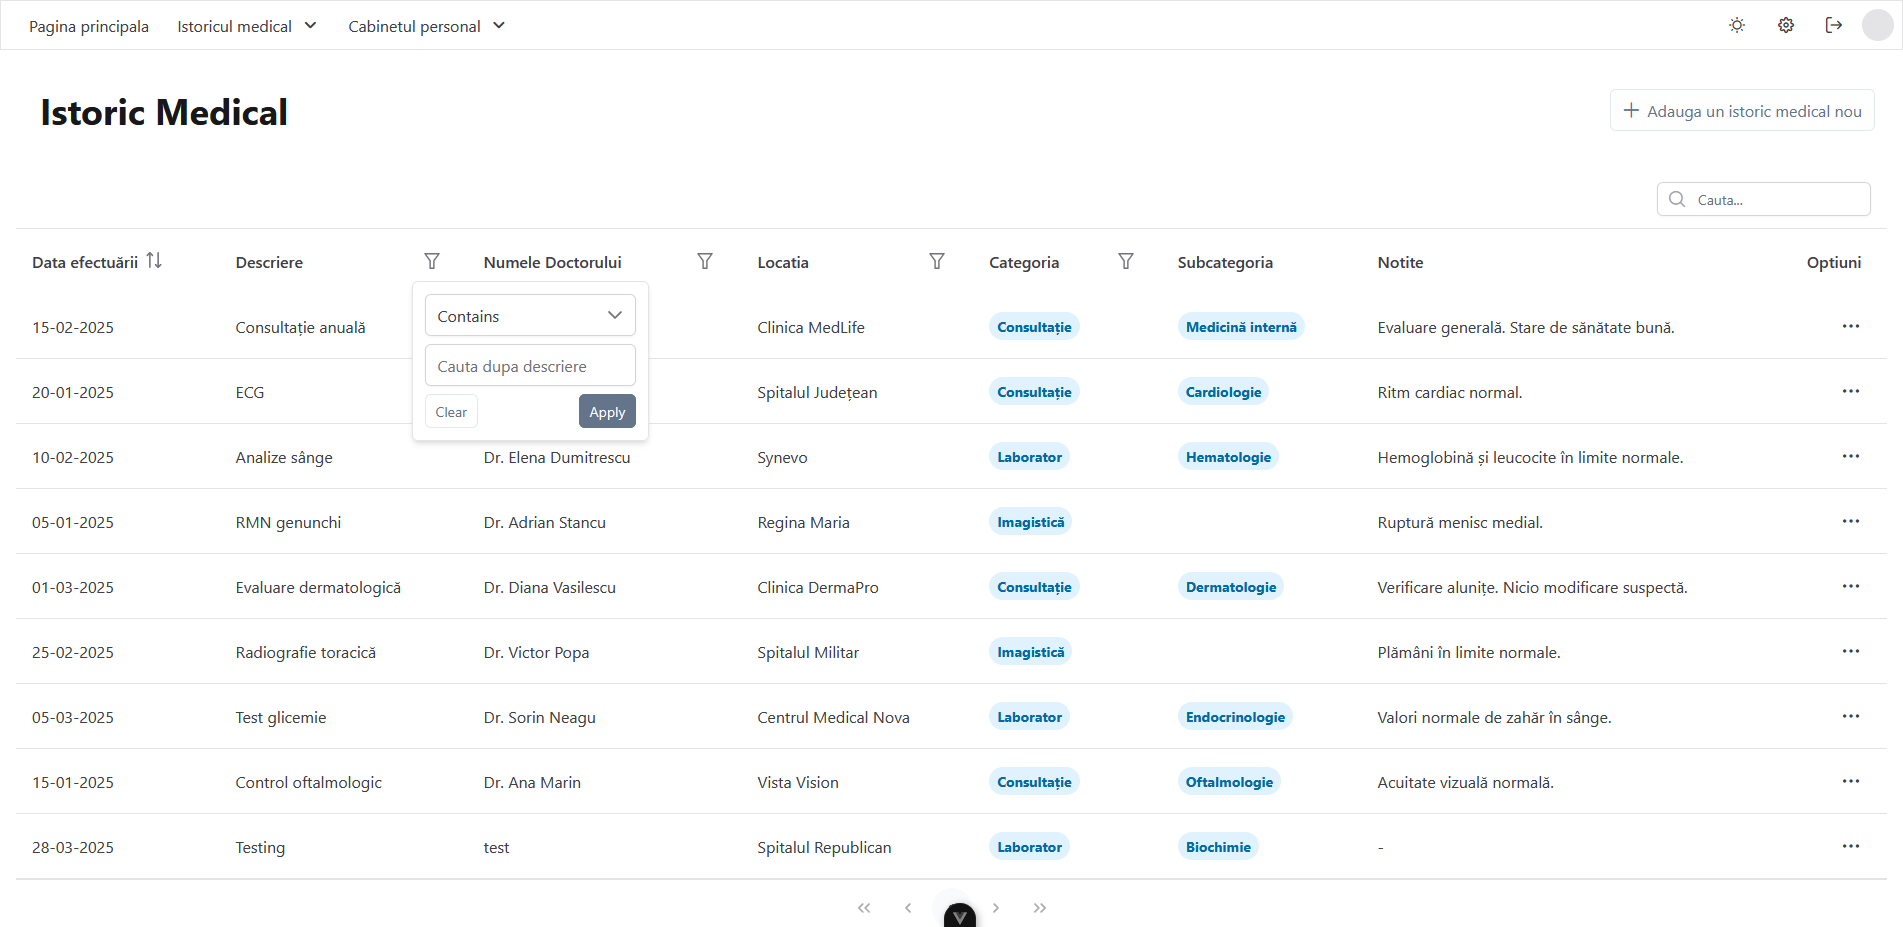
\includegraphics[width=\textwidth]{Desktop_HistoryView_Filter.png}
  \caption{Filter Menu for Health Records}\label{fig:filtermenu}
\end{figure}

\begin{lstlisting}[language=HTML, caption=Filter Function for Health Records]
  <template>
  <div class="h-full w-full px-4">
    <DataTable 
      v-model:filters="filters" 
      :value="history" 
      :rows="10" 
      paginator 
      dataKey="id" 
      filterDisplay="menu"
      :loading="loading"
      :globalFilterFields="['name', 'doctor_name', 'place', 'category']"
      removableSort
      responsiveLayout="stack"
      breakpoint="960px"
    >
      <template #header>
        <div class="flex justify-end">
          <IconField>
            <InputIcon>
              <i class="pi pi-search" />
            </InputIcon>
            <InputText size="small" v-model="filters['global'].value" placeholder="Cauta..." />
          </IconField>
        </div>
      </template>

      <!-- Previous columns here -->

      <Column field="doctor_name" header="Numele Doctorului" :showFilterMenu="true">
      <template #filter="{ filterModel, filterCallback }">
        <InputText v-model="filterModel.value" type="text" class="w-full" @input="filterCallback()" placeholder="Cauta dupa doctor" />
      </template>
    </Column>

    <!-- Next columns here -->
    </DataTable>
  </div>
</template>
\end{lstlisting}

Finally, with the addition of health records page, the ability to view and upload PDF files was also added to the system. This was an important feature to add, as files related to health records are usually sent in a PDF format. There was a slight challenge as to how to display the PDF files in the frontend, however in the end it was decided to use a simple approach that utilised in-built functionality through the use of object element from HTML. To allow mobile users to view the files, the system instead used a button to allow mobile users to download the file, as mobile browsers do not support the object element. The code for the PDF viewer can be seen below and a screenshot in figure~\ref{fig:pdfviewer}.

\begin{lstlisting}[language=HTML, caption=PDF viewer Function for Health]<template>
  <Dialog
    v-model:visible="visible"
    modal
    header="Vizualizeaza fisierul"
    class="w-full md:w-3/4 md:h-3/4"
    @hide="emit('close')"
  >
    <div v-if="metadata?.file_type == 'application/pdf'">
      <object
        :data="`http://localhost:8000/files/medicalhistory/${props.historyId}`"
        type="application/pdf"
        class="w-full h-[70vh] hidden md:block"
      />
      <div class="block md:hidden text-center mt-2">
        <a
          :href="`http://localhost:8000/files/medicalhistory/${props.historyId}`"
          target="_blank"
          class="bg-blue-500 text-white px-4 py-2 rounded-md inline-block mb-4"
        >
          Deschide certificatul PDF
        </a>
      </div>
    </div>
    <Image
      v-else
      :src="`http://localhost:8000/files/medicalhistory/${props.historyId}`"
      alt="Fisier consultatie"
      class="w-full h-screen"
      preview
    />
  </Dialog>
</template>
\end{lstlisting}

\begin{figure}[ht]
  \centering
  \subfloat[Desktop version]{%
      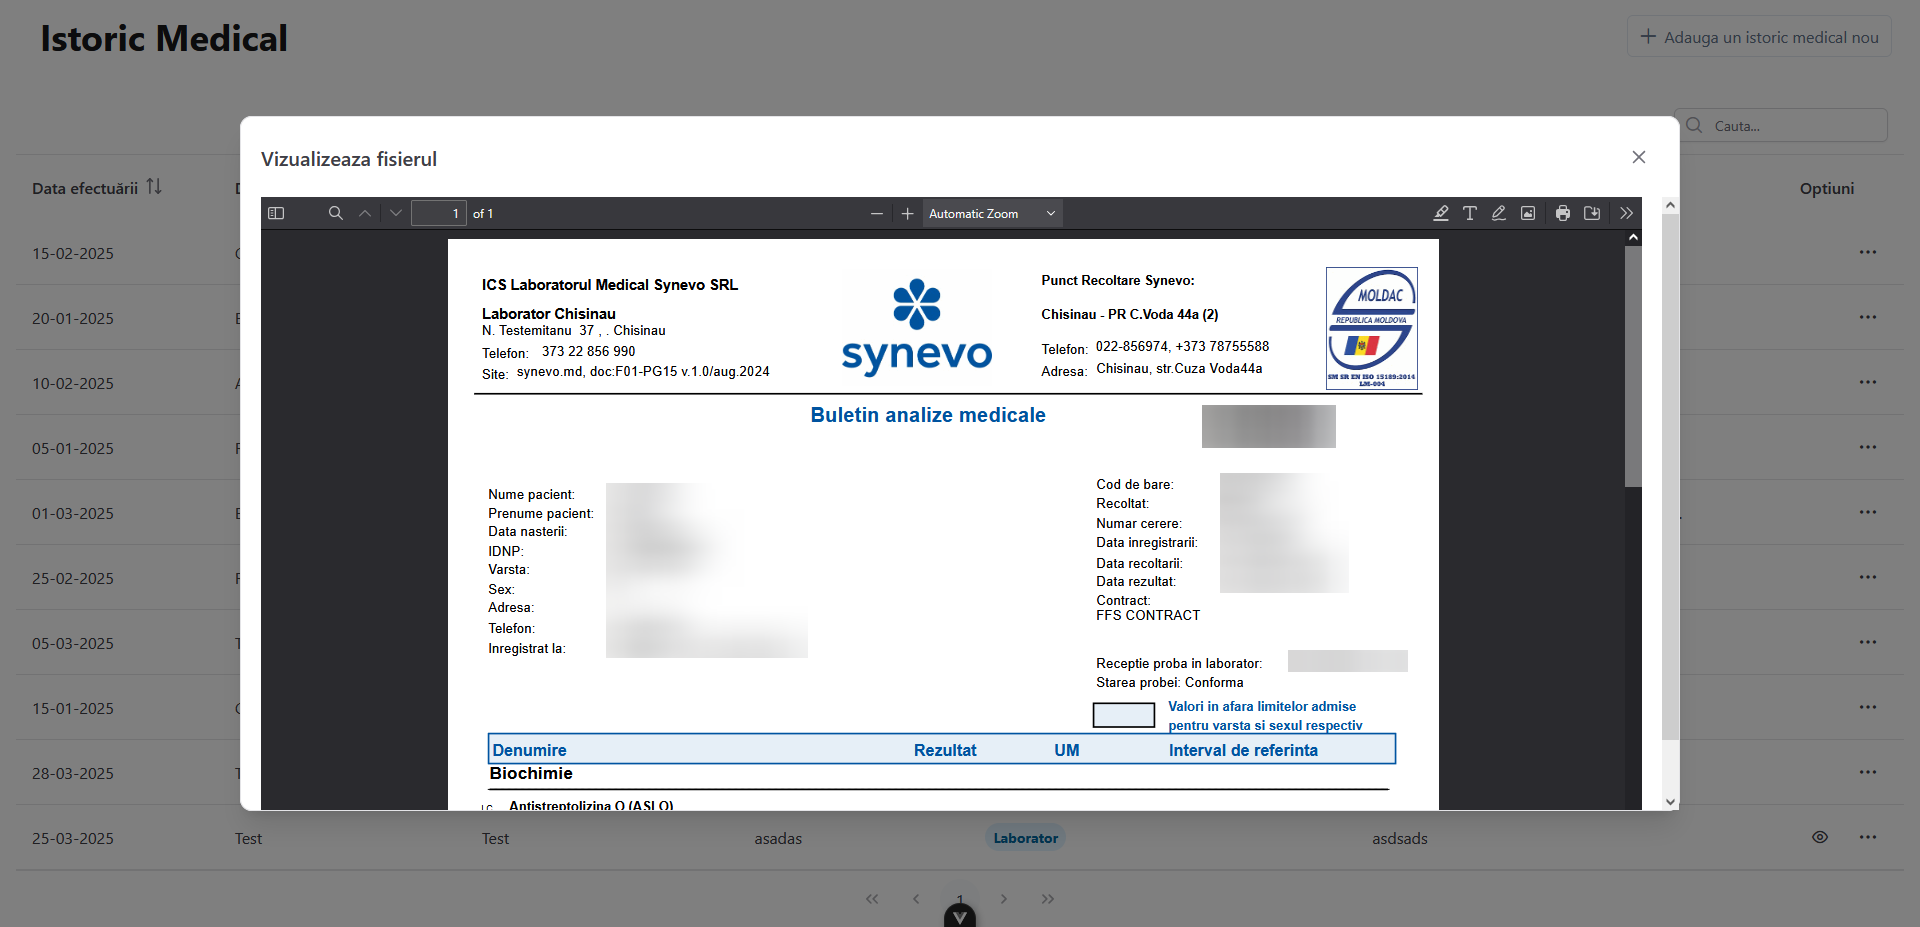
\includegraphics[width=\textwidth]{Desktop_History_PDF.png}%
  }
  \\[\baselineskip]
  \subfloat[Mobile version]{%
      
\includegraphics[width=0.4\textwidth]{Mobile_History_PDF.png}%
  }
  \caption{Desktop and Mobile version of the PDF viewer}\label{fig:pdfviewer}
\end{figure}

\FloatBarrier{}

\subsection{Backend changes}

To enable the health record functionality to work properly, new tables had to be created in the database to store the records: MedicalHistory for the main table, MedicalCategory for main categories of the records (lab tests, doctor consultations, etc) and additional tables like MedicalSubCategory and LabSubcategory for the subcategories of the records (blood test, urine test, etc). The new tables can be seen below in figure~\ref{fig:erd_s4}.

\noindent\begin{minipage}{\textwidth}
  \begin{center}
      \rotatebox[origin=c]{270}{
          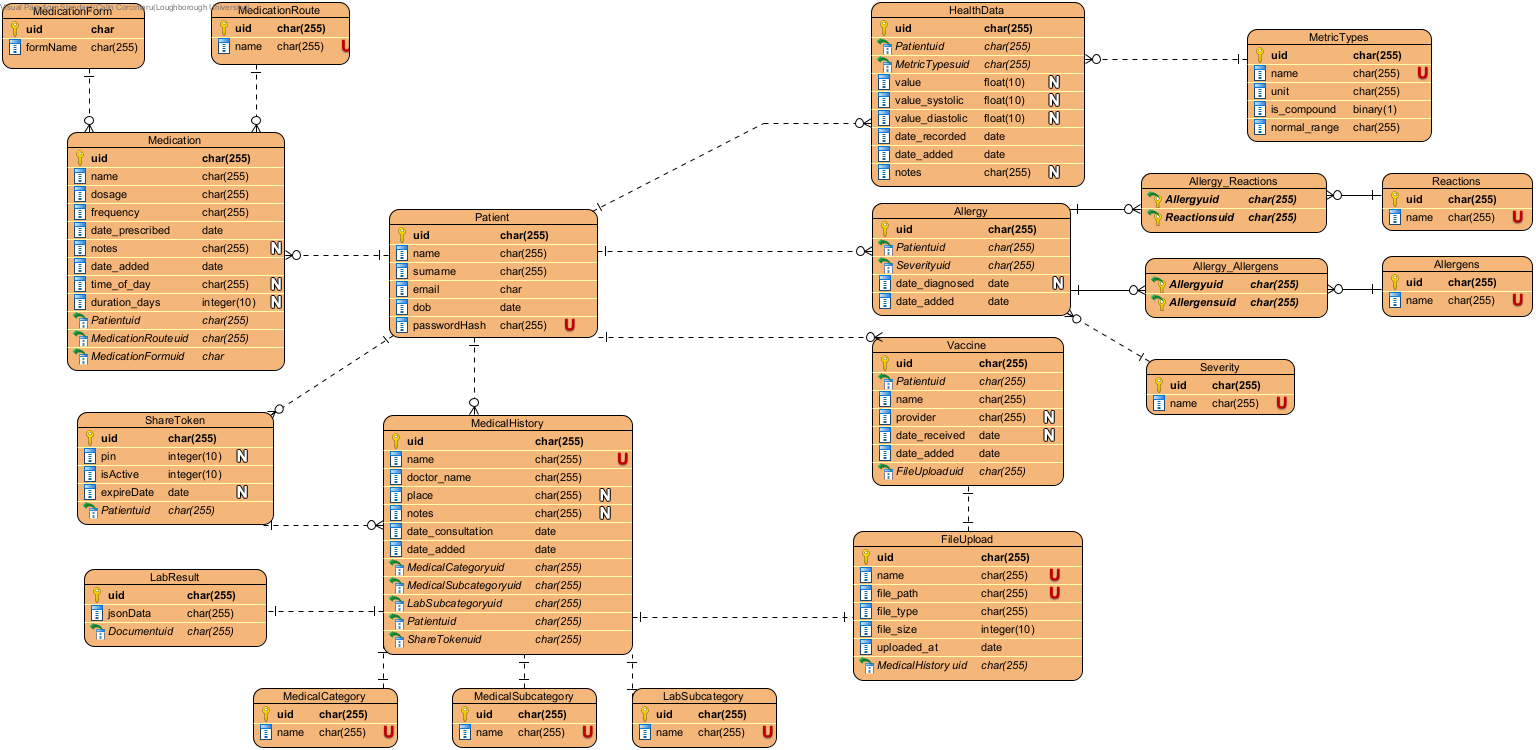
\includegraphics[width=0.95\textheight,keepaspectratio]{ERD_updatedS4.png}
      }
      \captionof{figure}{Updated Entity Relationship Diagram \- Sprint \#4}\label{fig:erd_s4}
  \end{center}
\end{minipage}

\FloatBarrier{}

Additionally, endpoints were created to allow the user to add, edit and delete health records. The endpoints were created in a similar way to the other endpoints in the system, using FastAPI and SQLModel.

\subsection{Work on stakeholder feedback}

As mentioned in the section introduction, in this sprint work was done to address the feedback received from stakeholder meetings regarding the features implemented in the previous sprint.

The biggest changes were related to how the vital signs are displayed and filtered in the system. The graph now shows lines for the upper and lower ranges for the respective vital signs, and a date range filter was added to the page, allowing the user to select a date range for the data displayed in the graph. 

Additionally, the most recent vitals are now compared to the normal range instead of the previous value. This change was implemented to ensure the normal range is used effectively to show whether their vitals signs are within or outside of it to allow for more informed decision making. These changes can be seen below in figure~\ref{fig:vitalchanges}.

\begin{figure}[htbp]
  \centering
  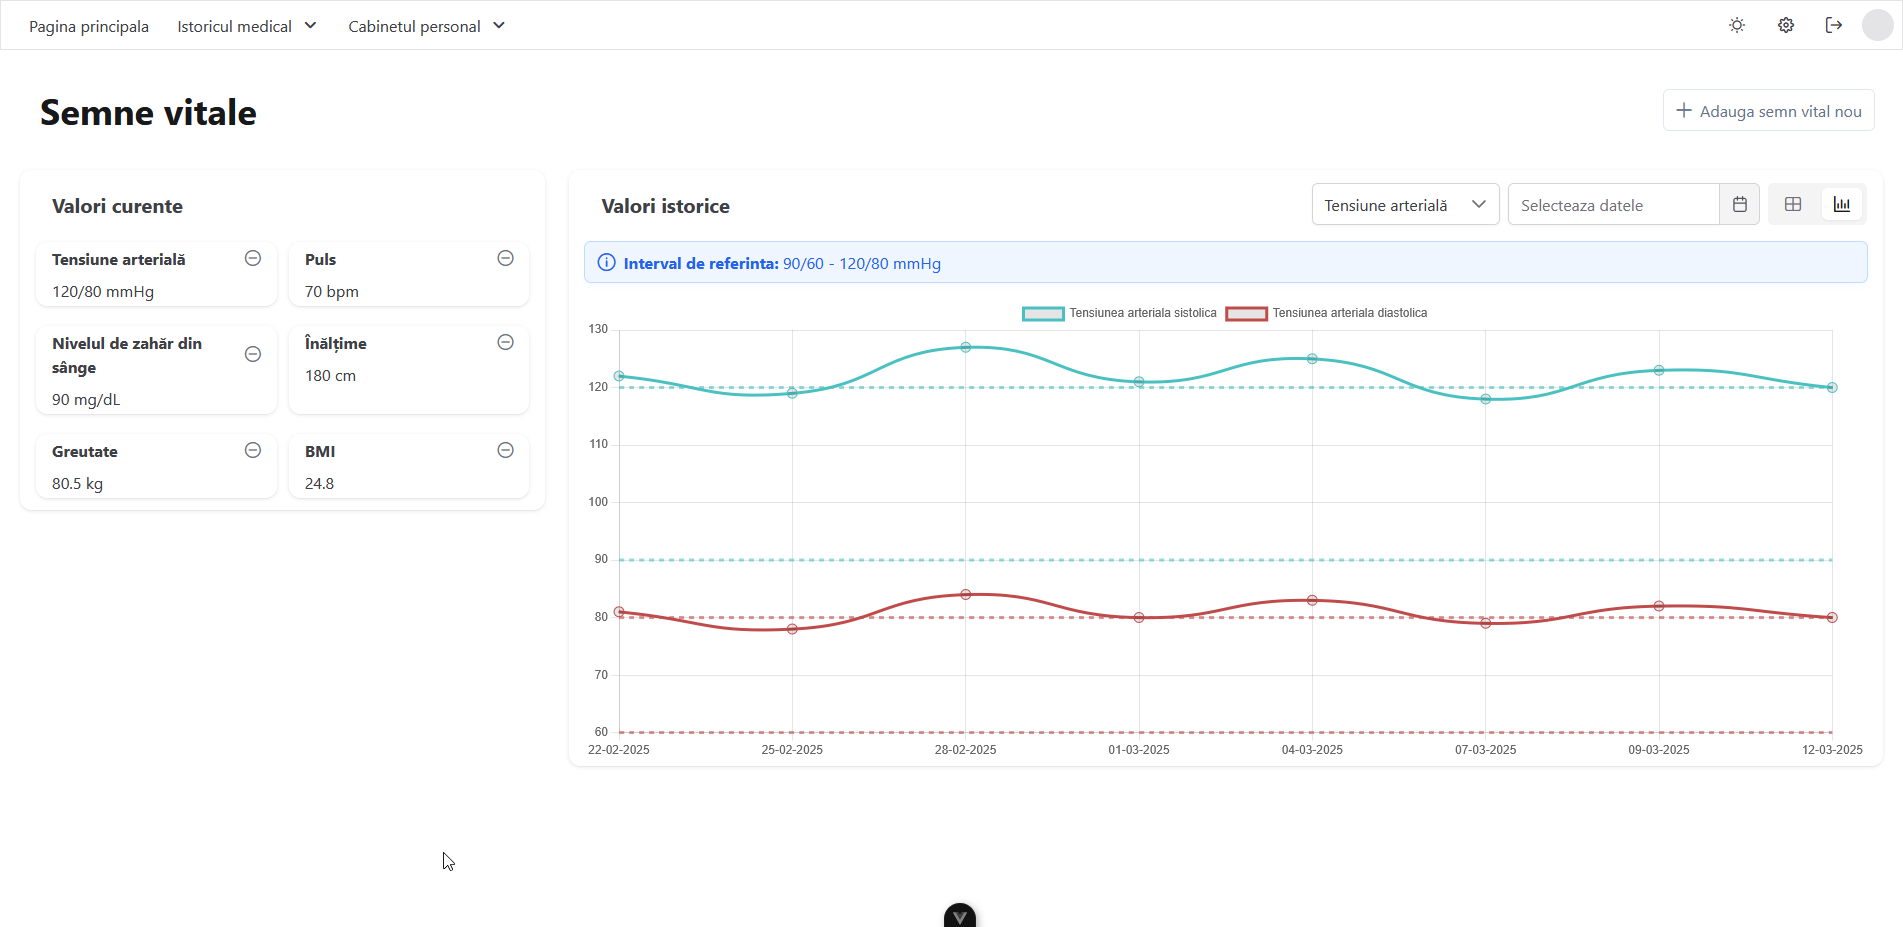
\includegraphics[width=\textwidth]{Desktop_Vitals_Updated.png}
  \caption{Updated Vitals View based on stakeholder feedback}\label{fig:vitalchanges}
\end{figure}

\FloatBarrier{}

The main dashboard page was also slightly changed to show the most recent vitals signs for each type of vital sign, instead of the most recent 5 values for each type. This was done to ensure that the dashboard page is not cluttered with too much information and that the user can easily see their most recent vitals signs.

Finally, the allergies section on the dashboard page was also changed to only show the moderate and severe allergies, as it was suggested by the stakeholders that this would be more useful for patients to track their most important allergies. The new dashboard can be seen below in figure~\ref{fig:dashboardchanges}.

\begin{figure}[htbp]
  \centering
  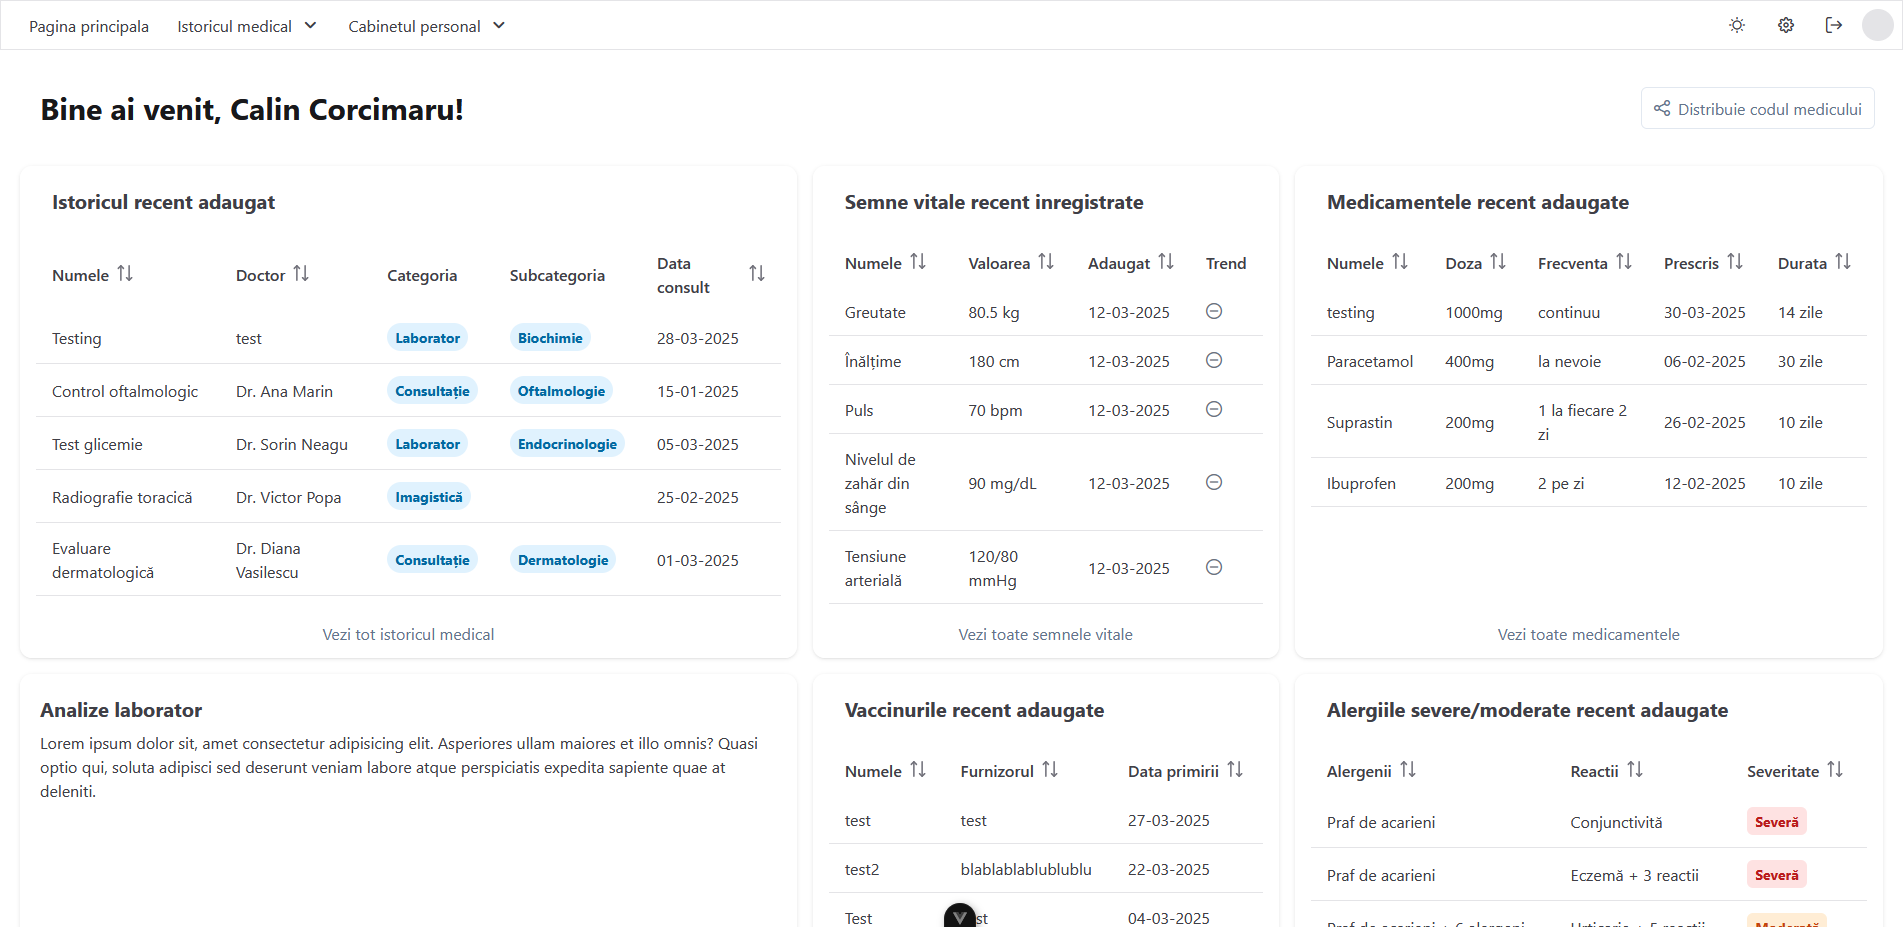
\includegraphics[width=\textwidth]{Desktop_DashboardView_Updated.png}
  \caption{Updated Dashboard View based on stakeholder feedback}\label{fig:dashboardchanges}
\end{figure}

\FloatBarrier{}

\subsection{Challenges}

The main challenge encountered in this sprint was actually not related to the project itself. Instead, the biggest challenge that was presented in this sprint was sickness, which led to the student being unable to work on the project for a week. This limited the amount of work that could be done in this sprint, leading to some of the preparatory work that was planned for this sprint to be moved to the next one.

\subsection{Requirements completed}

\begin{itemize}
  \item The system must allow the patient to specify and categorise the type of document they are uploading (lab test, doctor consultation, etc).
  \item The system must allow patients to upload their own medical records in a variety of formats (PDF, DOC, etc).
  \item The system must display the patient's history in a chronological order in the form of a timeline.
  \item When viewing doctor consultations, the system should divide them into categories based on the domain of the doctor (cardiology, neurology, etc).
  \item The system must allow the patient to add a description of the document they are uploading.
  \item The system should allow the patient to add a date for the document they are uploading.
  \item The system should allow the patient to add a location for the document they are uploading.
  \item The system should allow the patient to add the doctor name for the document they are uploading.
  \item The system should allow the patient to sort and filter the documents based on the type of document, date, location, and doctor name. 
\end{itemize}

\section{Sprint \#5}

The fifth sprint of the project was focused on adding the ability to add lab tests and extract the lab result values from those documents. The lab results would've been extracted by using a multimodal LLM, which would allow the system to precisely collect the lab results alongside other information such as units, reference ranges, etc without any additional human or system intervention. Using a MLLM would also simplify the extraction as the model would be able to export the results in an easily parseable response, such as JSON, which could be then used to display the information on the frontend or be processed in the backend. This feature was probably one of the most important ones in the whole system, as it represented an innovative way of automating the collection and storage of lab results for patients.  

This feature was a continuation of the work done in the previous sprint, as the lab tests were also part of the health records feature. As such, some of the initial work was done on top of existing components, which made development easier and faster. The feature was developed as per the initially agreed requirements and wireframes, with some changes to how the lab results were displayed on the frontend.

The sequence diagram for the lab tests extraction can be seen below in figure~\ref{fig:sequence_lab}. The diagram shows how the user interacts with the system to upload a lab test, how the system processes the file and sends it to the MLLM API, and how the response is then displayed to the user.

\begin{figure}[htbp]
  \centering
  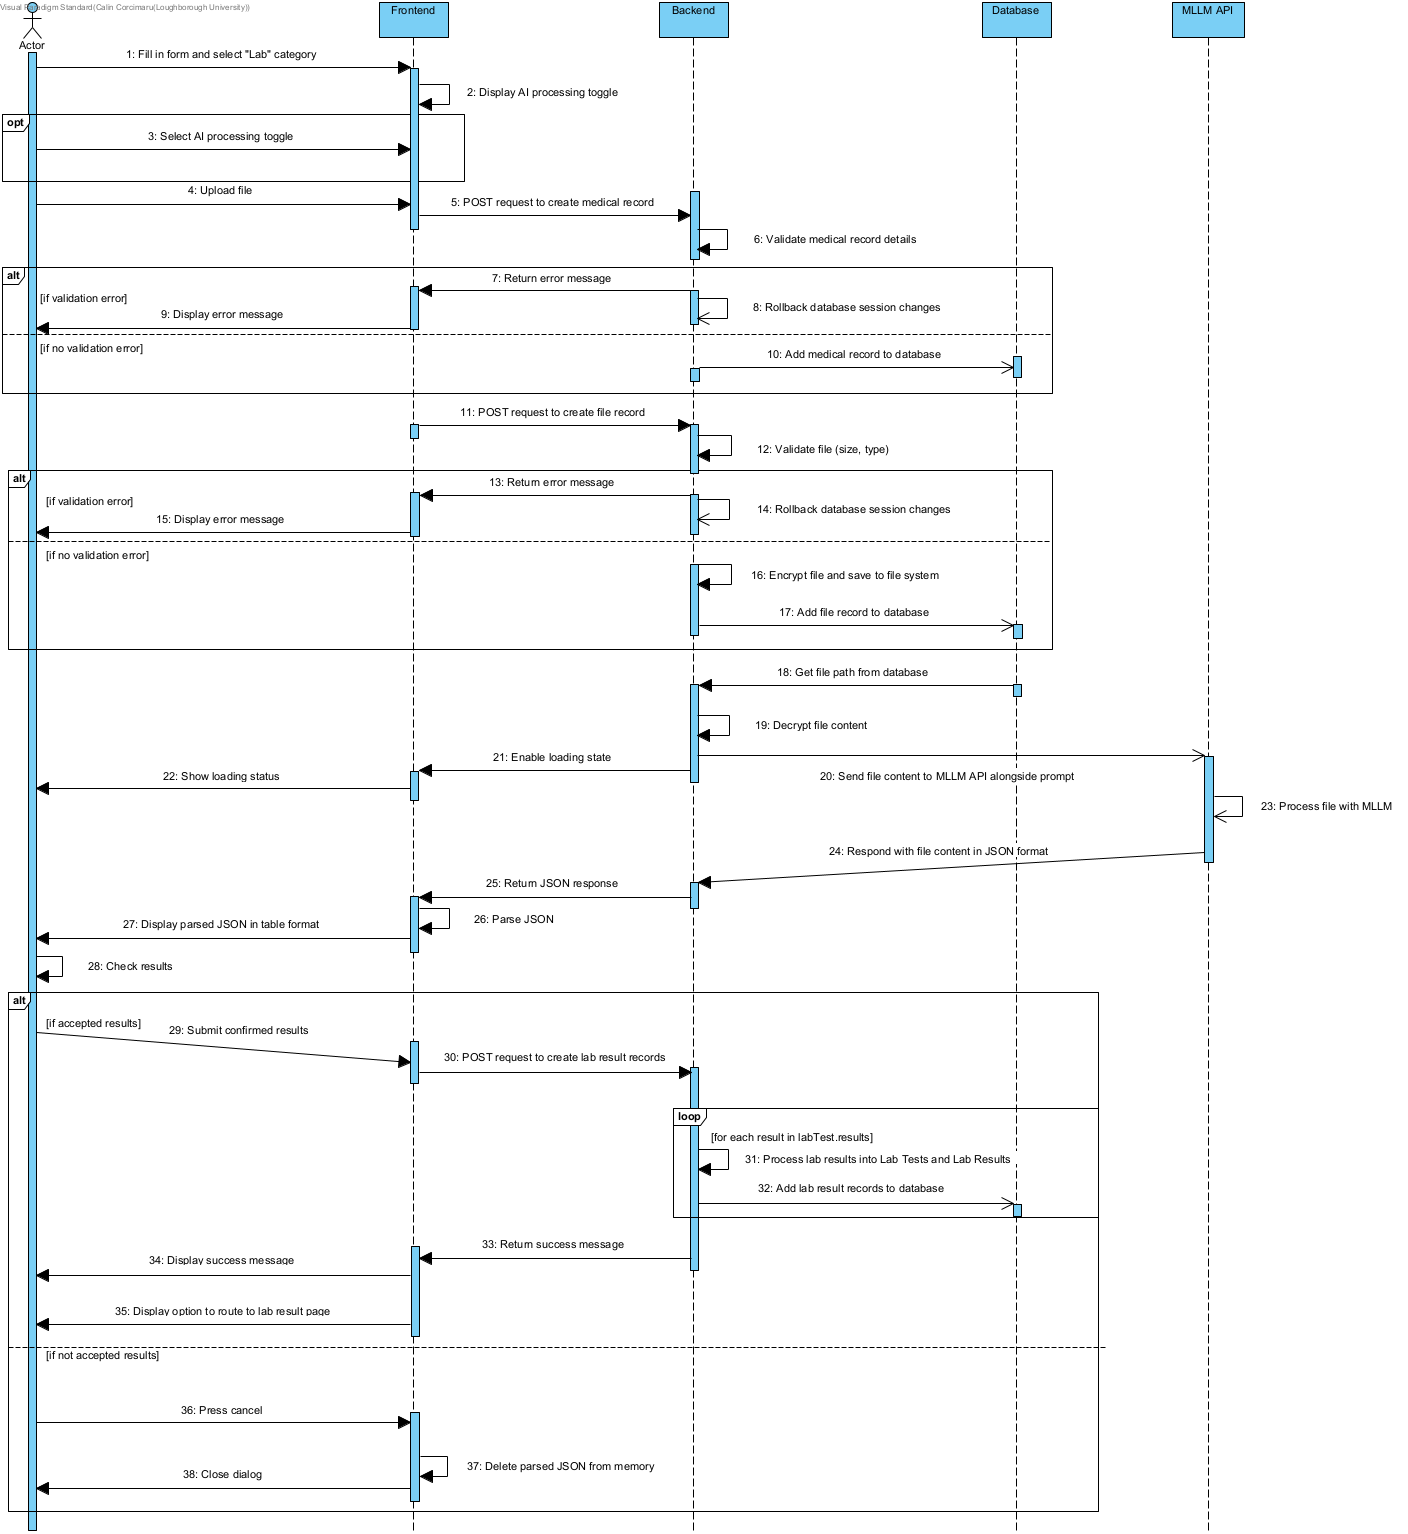
\includegraphics[width=\textwidth,height=0.8\textheight,keepaspectratio]{Sequence_lab.png}
  \caption{UML Sequence Diagram --- Extracting Lab Results}\label{fig:sequence_lab}
\end{figure}

\subsection{Lab Tests Extraction}

As lab tests were previously added in sprint \#4 as a health record, it was decided to use the existing `Add Health Record' component to allow the user to choose whether they'd like to extract the lab results besides uploading the file to the system. The decision was made to streamline the user experience of adding new health records, as the user would not have to go through multiple steps to add a lab test, but also because it would speed up development time as an existing component could be reused and made more feature-rich. Finally, this also closely matched the initial wireframe design for the `New Document' dialog, which can be seen in figure~\ref{fig:newDoc_wireframe}.

The updated dialog can be seen below in figure~\ref{fig:labs_addDoc}. The main change that can be seen is the addition of a toggle switch, which is displayed only when the user selects a lab test as the document type. If used, the toggle would still send the lab file to the backend and save it as a health record, but in addition to this, it would also send it to the MLLM API to be processed. 

\begin{figure}[ht]
  \centering
  \subfloat[Desktop version]{%
      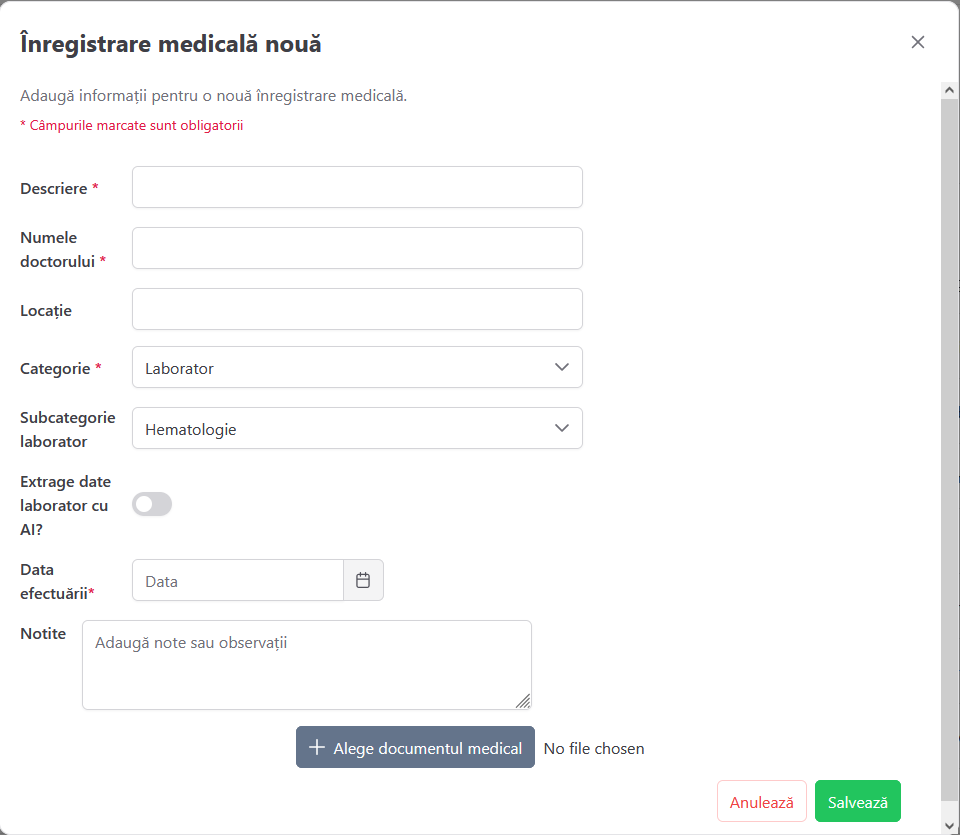
\includegraphics[width=0.7\textwidth]{Desktop_AddDoc_Labs.png}%
  }
  \\[\baselineskip]
  \subfloat[Mobile version]{%
      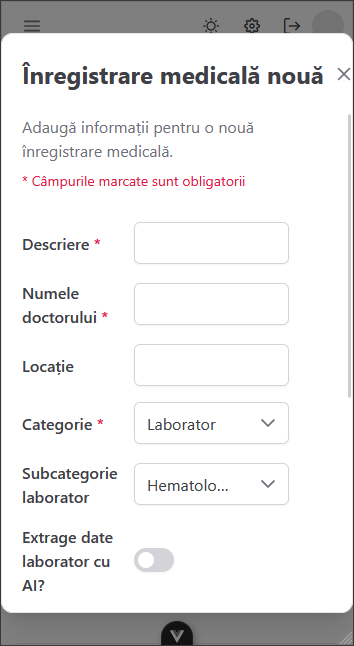
\includegraphics[width=0.3\textwidth]{Mobile_AddDoc_Labs.png}%
  }
  \caption{Desktop and Mobile version of the new Add Document dialog}\label{fig:labs_addDoc}
\end{figure}

\FloatBarrier{}

After the record is created and file is uploaded, the backend would find the file and send it the MLLM API\@. This was done to avoid uploading the file twice and to ensure the file would be successfully uploaded to the system before sending to the API\@.

The MLLM chosen for this project was Google's Gemini 2.0 Flash, which, as of writing this section, is part of the newly released family of Gemini models \parencite{gemini2}\@. The choice was made based on the list of available MLLMs that can be accessed via APIs with a free tier from table~\ref{tab:llm_apis}. Besides Google's AI Studio, none of the API providers allowed the uploading and processing of files, which made Gemini 2.0 Flash the most suitable choice for the project. It was noted that a local MLLM could've also been used for the project, a point which will be discussed in more detail in section~\ref{sec:future_work}.

Because an API was used, most of the work with the MLLM involved using Prompt Engineering techniques to ensure the model would process and return the data in the desired format. Prompting techniques from previous section~\ref{sec:prompt} were used to write the following prompt that was used to extract the lab results from the file:

\begin{lstlisting}[language=Python, caption=Prompt for Lab Results Extraction]

def extract_with_llm(file_content: bytes, file_type: str):
  prompt = """
  You have been given a document that contains lab results that is written in the Romanian language. Your job is to extract all lab results from this document in JSON format with the following fields: test_name, test_code, value, unit, reference_range, method. Sometimes the code of the test will be in the name itself, and it is your job to determine if the code is there, for example in brackets or separated by a comma, and separate the name and the code. Sometimes the lab result will not have a method specified, and in that case you return an empty string. The document is in Romanian, however the JSON keys should be in English.

  EXTREMELY IMPORTANT FORMATTING INSTRUCTIONS:
  1. Return ONLY the raw JSON array
  2. DO NOT use code blocks, backticks, or markdown formatting
  3. DO NOT include ```json or ``` anywhere in your response
  4. DO NOT include any explanations or text before or after the JSON
  5. Your response must start with the '[' character and end with the ']' character
  6. The output should be valid JSON that can be parsed directly
  7. Use period (.) as the decimal separator, not comma (,)

  Example of how your output should look, starting from the very first character:
  [{"test_name":"Hemoglobina","test_code":"HGB","value":"14.3","unit":"mg/dL","reference_range":"13.2-17.3", "method":"Chemiluminiscenta"}]
  
  if there is no method specified, return an empty string:
  [{"test_name":"Hemoglobina","test_code":"HGB","value":"14.3","unit":"mg/dL","reference_range":"13.2-17.3", "method":" "}]
  """
  
  response = client.models.generate_content(
      model="gemini-2.0-flash",
      contents=[prompt,
              types.Part.from_bytes(
              data=file_content, 
              mime_type=file_type
              )
          ])
  
  return response.text
  
\end{lstlisting}

The response from the API would be a JSON array containing all the lab results extracted from the document. Before saving, it is important to make sure the results and their values are correct. As such, it was decided to display all the extracted results back to the user in a PrimeVue DataTable component, which allowed for easy filtering of the results, but also for row-based editing. This way, the user could easily edit the values or remove any unwanted results before saving them to the system. An example of how the extracted lab results dialog looks can be seen below in figure~\ref{fig:labs_extracted}.

\begin{figure}[htbp]
  \centering
  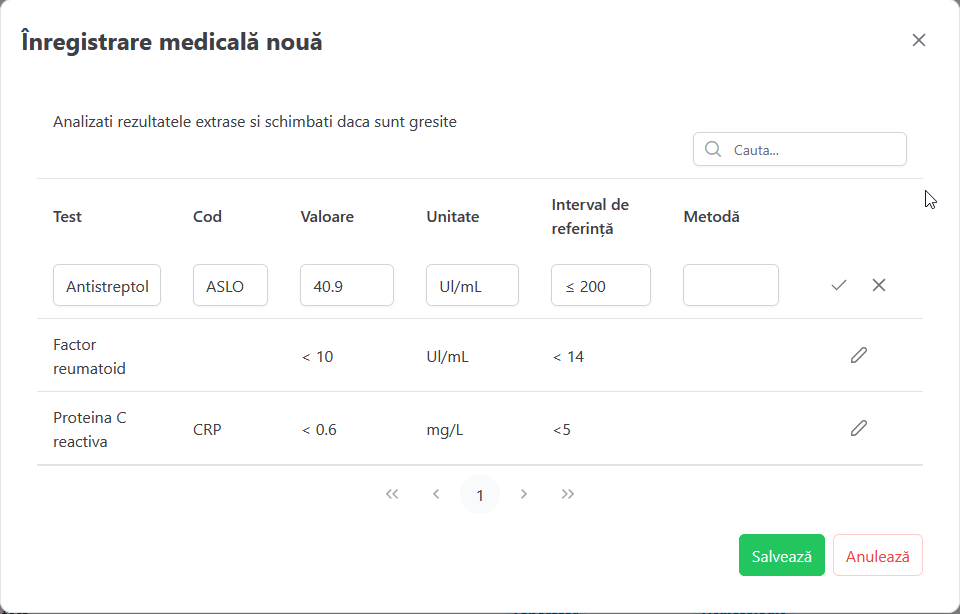
\includegraphics[width=\textwidth]{Desktop_Validate_Labs.png}
  \caption{Desktop dialog validation of extracted lab results}\label{fig:labs_extracted}
\end{figure}

A benefit of using PrimeVue's DataTables was not only its row editing feature or its filtering options, but also its ability to dynamically create columns based on the data received. This was perfect for the lab results, as it is not possible to know beforehand how many results will be extracted from a document. A code snippet of the DataTable can be seen below:

\begin{lstlisting}[language=HTML, caption=Dynamic DataTable for Lab Results]
  <DataTable
    :value="extractionResult"
    v-model:editingRows="editingRows"
    class="w-full"
    :rows="10"
    editMode="row"
    paginator
    dataKey="test_name"
    @row-edit-save="onRowEditSave"
    v-model:filters="filters"
    :globalFilterFields="['test_name', 'test_code']"
  >
    <template #header>
      <h2 class="m-0">Analizati rezultatele extrase si schimbati daca sunt gresite</h2>
      <div class="flex justify-end">
        <IconField>
          <InputIcon>
            <i class="pi pi-search" />
          </InputIcon>
          <InputText
            size="small"
            v-model="filters['global'].value"
            placeholder="Cauta..."
          />
        </IconField>
      </div>
    </template>
    <Column 
      v-for="col of columns" 
      :key="col.field" 
      :field="col.field" 
      :header="col.header"
    >
      <template #editor="{ data, field }">
        <InputText v-model="data[field]" class="w-full" fluid />
      </template>
    </Column>
    <Column
      :rowEditor="true"
      style="width: 10%; min-width: 8rem"
      bodyStyle="text-align:center"
    />
  </DataTable>
\end{lstlisting}

After confirming the extracted test results, they are processed and saved to the backend. The next subsection will discuss in more detail how the backend was changed to accommodate the new lab tests and their results.

\subsubsection{Backend changes}

To supporrt the processing and addition to database for the newly extracted lab results, two new tables were created in the database: LabTest and LabResult. The decision to use 2 tables was made to avoid duplication of data for fields like name and code of the lab test, as these would be common for all the lab results, regardless of their method or machinery used. This would also prove beneficial as multiple results could be assigned to one test, making the tracking and display of the historical results much easier. Finally, by having 2 separate tables, LabTests could be dynamically populated with new tests straight from uploaded documents, without the need for manual addition or creation of test types. The updated database schema can be seen below in figure~\ref{fig:erd_s5}.

\noindent\begin{minipage}{\textwidth}
  \begin{center}
      \rotatebox[origin=c]{270}{
          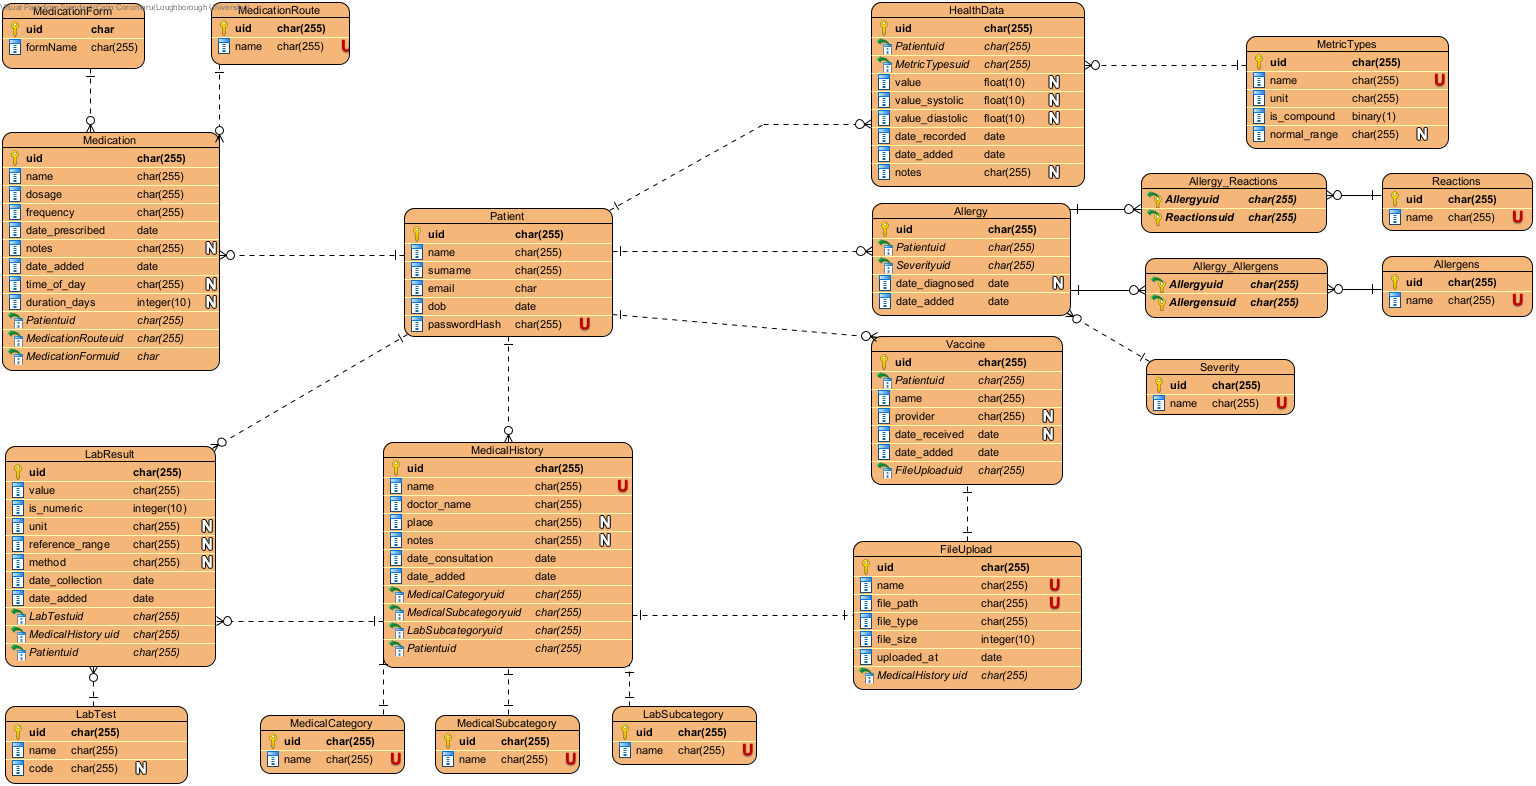
\includegraphics[width=0.95\textheight,keepaspectratio]{ERD_updatedS5.png}
      }
      \captionof{figure}{Updated Entity Relationship Diagram \- Sprint \#5}\label{fig:erd_s5}
  \end{center}
\end{minipage}

\FloatBarrier{}

As can be seen by the diagram above, there might seem to be a redundant relationship between the Patient and LabResult tables, as LabResult is already related to MedicalHistory, which in turn is related to a Patient. However, the decision was made to introduce the relationship as it would allow for easier querying when getting all the lab results for a patient, in the case of the dashboard view or even in the next sprint when the share functionality is added.

Similarly, a code snippet of the endpoint that handles the creation of lab results can be seen below:

\begin{lstlisting}[language=Python, caption=Lab Results Endpoint]
  # Create the lab test records in the database
@router.post('/me/labtests/')
async def create_lab_tests(extraction_result: LabsCreate, user_id: uuid.UUID = Depends(validate_session), session: Session = Depends(get_session)):
    medhistory = session.get(MedicalHistory, extraction_result.medicalhistory_id)
    user = session.get(User, user_id)
    
    if not medhistory:
        raise HTTPException(status_code=status.HTTP_404_NOT_FOUND, detail="Medical history not found")
    
    if medhistory.user_id != user_id:
        raise HTTPException(status_code=status.HTTP_403_FORBIDDEN, detail="Not authorized to access this medical history")
    
    for lab_item in extraction_result.lab_tests:
        lab_test = session.exec(select(LabTest).where(LabTest.name == lab_item.name)).first()
        
        if not lab_test:
            lab_test = LabTest(
                name = lab_item.name,
                code = lab_item.code,
            )
            session.add(lab_test)
            session.flush()
        
        lab_result = LabResult(
            value = lab_item.value,
            is_numeric = check_is_numeric(lab_item.value),
            unit = lab_item.unit,
            reference_range = lab_item.reference_range,
            date_collection = extraction_result.date_collection,
            test = lab_test,
            medicalhistory = medhistory,
            user = user,
            method = lab_item.method
        )
        
        session.add(lab_result)
        session.flush()
        
    session.commit()
    
    return {
        "status": status.HTTP_201_CREATED,
        "message": "Lab tests created successfully"
        }
\end{lstlisting}

\subsection{Lab Results Display}

The final part of the work on the lab extraction feature was the display of said results within their own page in the system. The initial idea was to reuse the existing design from the vitals page, which can be seen in figures~\ref{fig:vitalspage},~\ref{fig:vitalspagegraph} and~\ref{fig:vitalchanges}. This would've also followed the initially agreed wireframes and design. 

However, upon discussing with stakeholders, an idea and request to change the design was floated in the meeting: instead of using the design from vitals page, the idea was to display everything in a tabular format where rows could be expanded to show the historical resutls from that specific test. This is where the division into 2 tables in the database played an important role: LabTest could be used as the `parent' element in the table, which could be sorted and filtered, while the LabResult elements would only be shown if the row would be expanded in the table. 

This idea was eventually accepted, as it would allow for a more compact view of the lab results, easier filtering/sorting and it enabled for a way to display the most recent results for each test as a separate column without being intrusive. The results were sorted by date in the backend already, which allowed for the most recent results to be easily selected and displayed. Finally, instead of using a big graph that might take up a lot of space on the page, it was decided to use a small graph, also known as a sparkline, which would only show the trend of the results over time, based on their reference range and collection date. Colors such as red and green were used to indicate whether the results were within the normal range or outside of it. An example of how the new lab results page looks can be seen below in figure~\ref{fig:labs_page} and~\ref{fig:labs_page_mobile}.

\begin{figure}[ht]
  \centering
  \subfloat[Desktop version]{%
      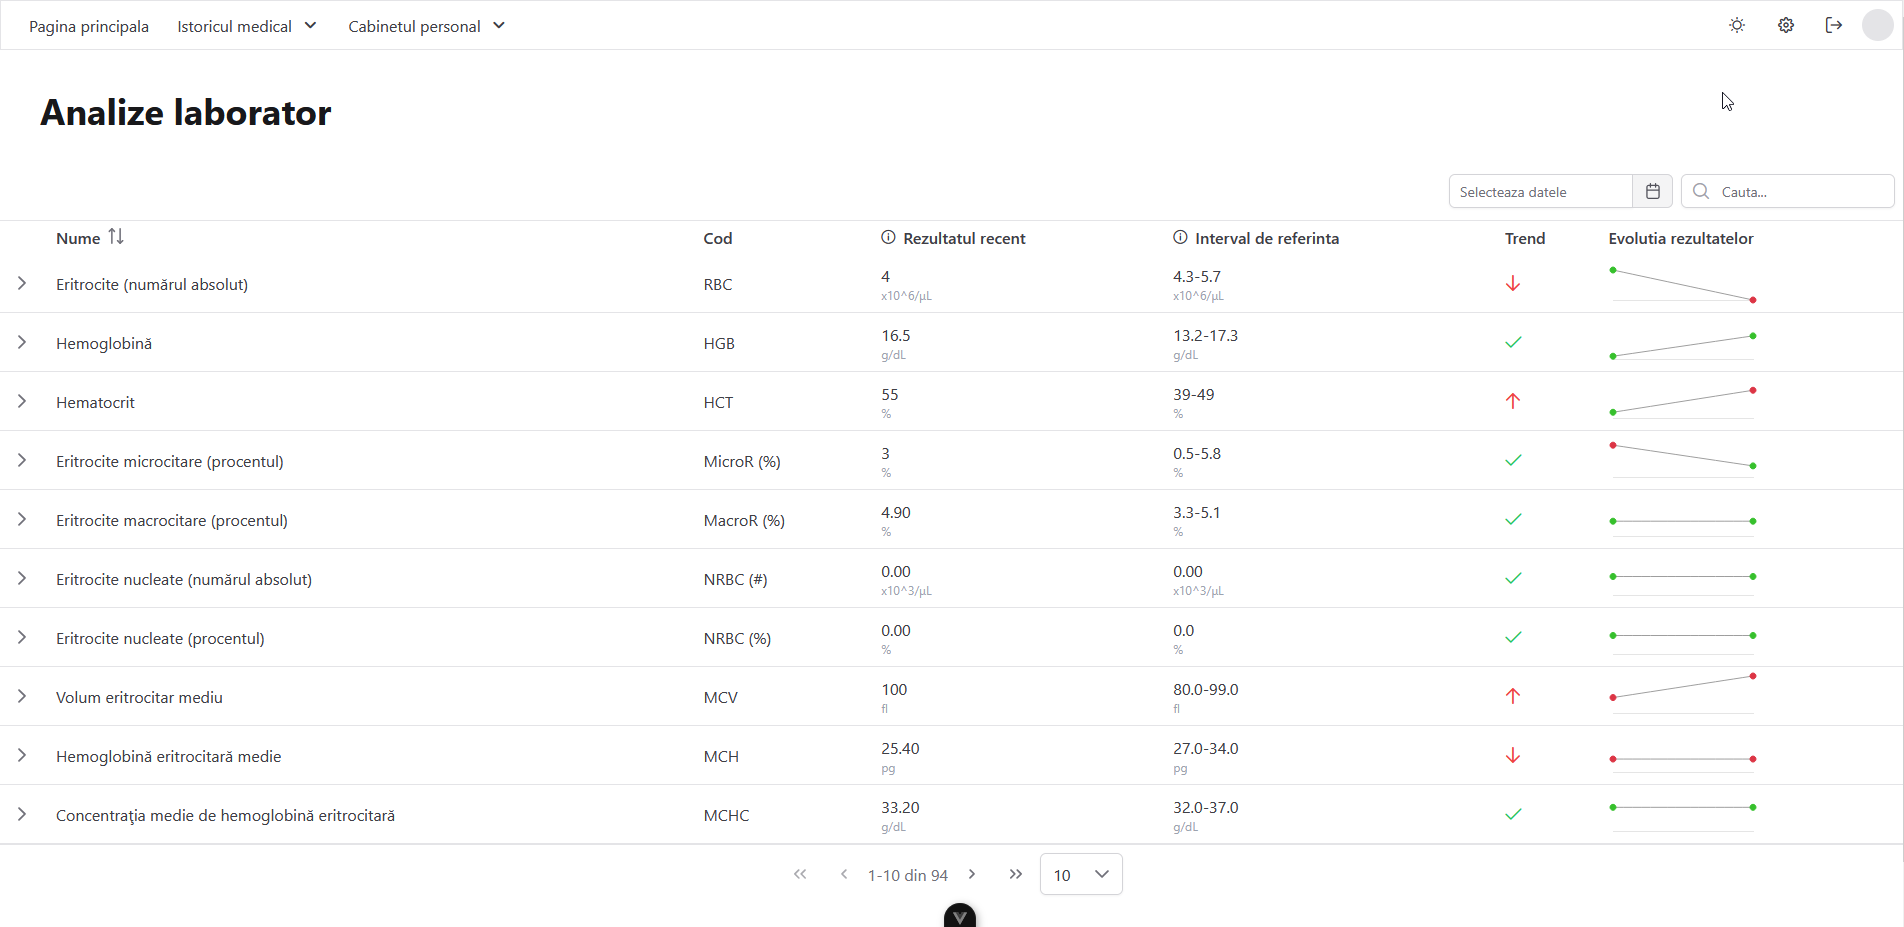
\includegraphics[width=0.9\textwidth]{Desktop_LabView.png}%
  }
  \\[\baselineskip]
  \subfloat[Desktop version \#2]{%
      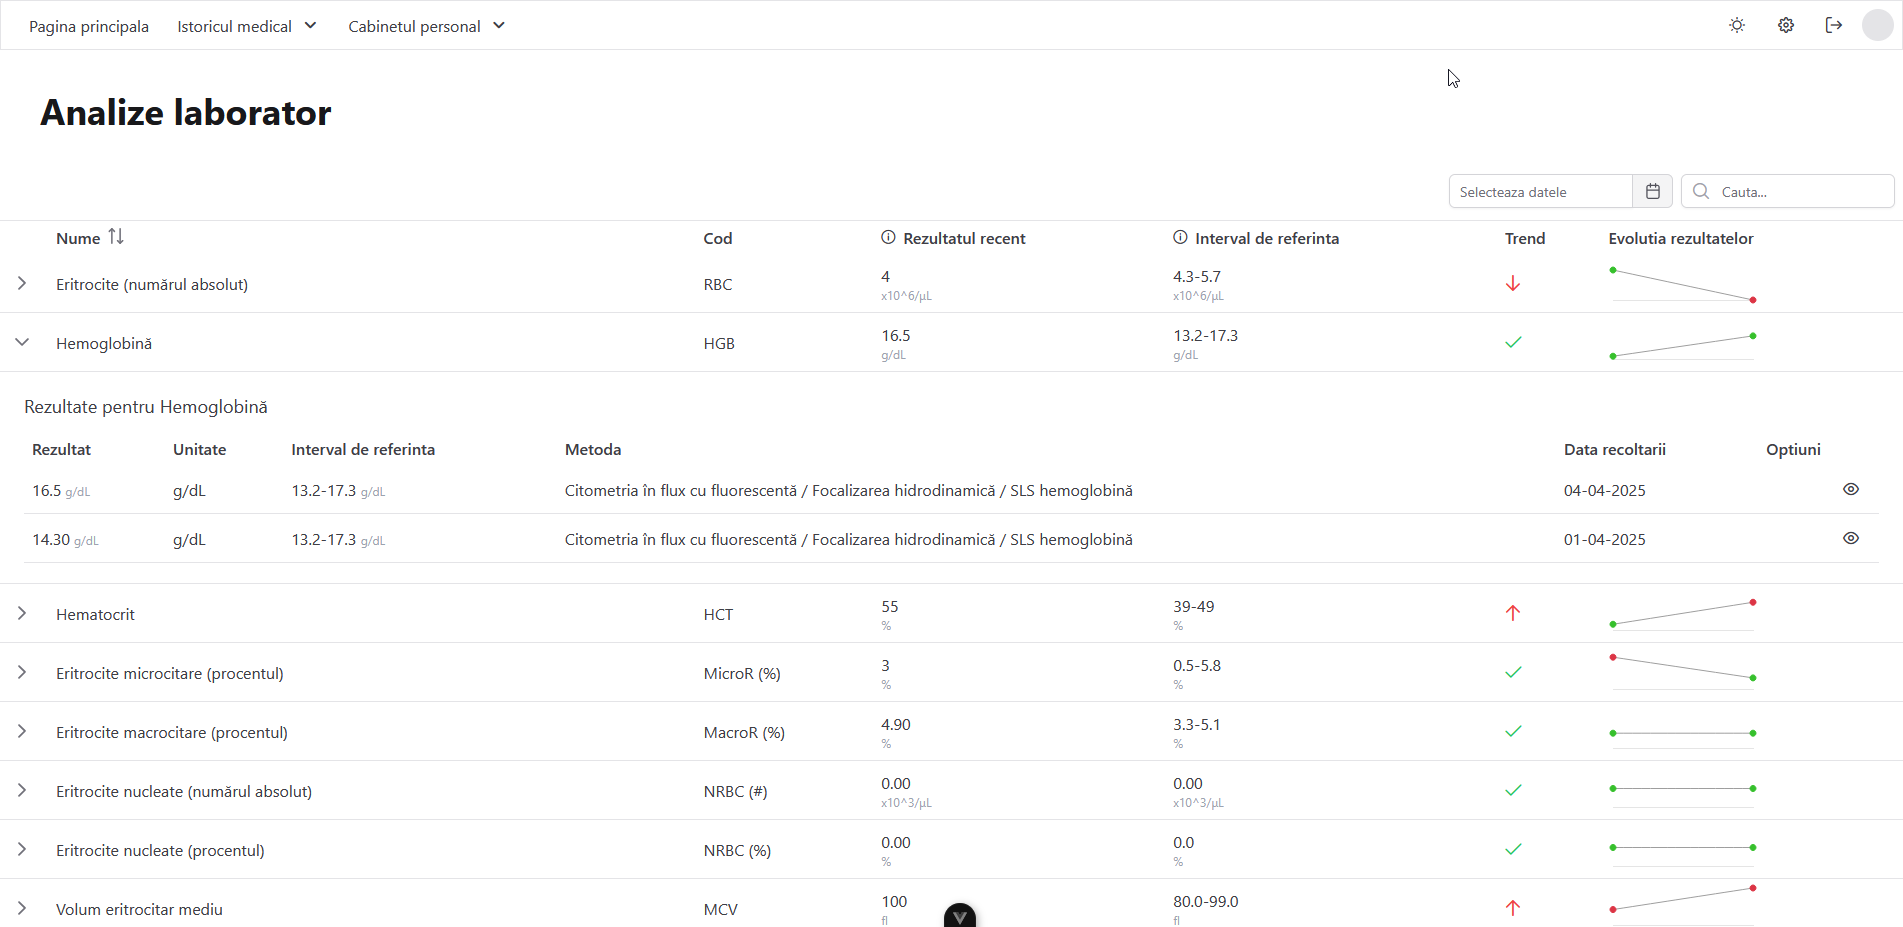
\includegraphics[width=0.9\textwidth]{Desktop_LabView2.png}%
  }
  \caption{Desktop version of the new Lab View page}\label{fig:labs_page}
\end{figure}

\FloatBarrier{}

\begin{figure}[ht]
  \centering
  \subfloat[Mobile version]{%
      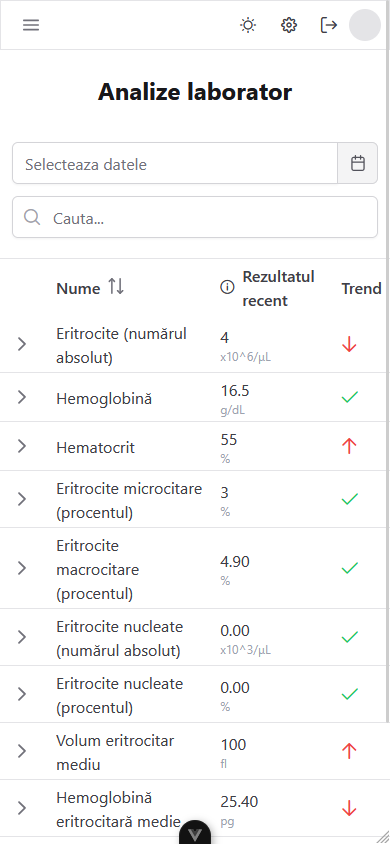
\includegraphics[width=0.4\textwidth]{Mobile_LabView.png}%
  }
  \hfill
  \subfloat[Mobile version \#2]{%
      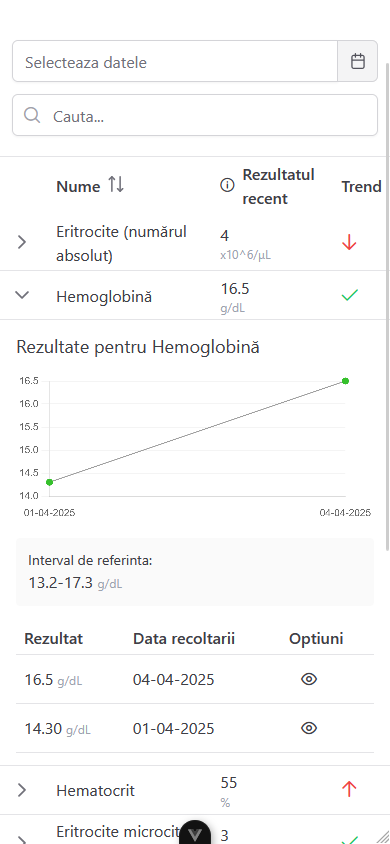
\includegraphics[width=0.4\textwidth]{Mobile_LabView2.png}%
  }
  \caption{Mobile version of the new Lab View page}\label{fig:labs_page_mobile}
\end{figure}

\FloatBarrier{}

\subsection{Challenges encountered}

This sprint encountered less challenges than the previous ones, meaning that the work was able to be done faster than it was initially planned. However, there were still some challenges that were encountered during the development of the lab tests extraction feature.

One of the biggest challenges was the change in design for the lab results page. Even though the initial design was agreed upon before the development begun, the stakeholders insisted on the change in design, which added a slight overhead in the form of additional design and research on how to implement the new idea. However, it must be noted that the new design also allowed for an easier development experience as a lot of the work was done by PrimeVue's DataTable component, which ultimately sped up the completion of the feature. Ultimately, the agility of the development process allowed for the change to be made without any major issues, an idea which will be further discussed in section~\ref{sec:future_work}.

The other challenge was the time pressure, as the student was nearing the deadline of the project. This meant that the focus was on implementing only the most necessary and basic features, without any space for creative or innovative ideas.

\subsection{Requirements completed}

\begin{itemize}
  \item The system must provide an overview of the patient history through 3 main sections: personal information, lab tests, and doctor consultations.
  \item The system must allow the doctor to view blood tests in a graphical format.
  \item The system must allow the doctor to view blood tests in a numerical, tabular format.
  \item The system must allow the doctor to view the patient's history in a chronological order.
  \item For blood test results, the system should display the normal range values for each test.
  \item The system could allow the patient to switch between viewing the lab tests in the document format or in a tabular, numerical format.
\end{itemize}

\section{Sprint \#6}

The last sprint of the project was focused on adding the ability to share the health records with doctors. This was one of the most important features of the system, as it allowed patients to share their medical history with doctors, which was one of the system's main goals of solving the problem of having so many different institution and systems that silo the patient information, without a way to share it. 

The purpose of the share link feature was to allow doctors to access the patient's accrued medical history during consultations. It is not aimed to replace their institutions' systems, but rather as a complimentary service that would enable them to view information that might not be available to them, thus creating a more complete picture of the patient's medical history.

This was the hardest feature to implement, as it would combine all the work done in the previous sprints and required designing a way to create these shareable links that would be both secure and easy to use.

\subsection{Share links}

In the initial discussions with stakeholders, it was quickly established that the easiest way to share medical information with healthcare practitioners would be through the use of a shareable link. Since most doctors have access to internet and a computer at their desks, it would represent the fastest and easiet way to access this system. Share links are also very versatile, as they could be sent via email, written on a paper, dictated or even generated as a QR code that can be scanned. As such, one of the first challenges was to design these shareable links so that they would be easy to transmit, but also secure and not easily guessable.

Initially, the idea was to use UUID as the share code, as their length (usually around 36 characters) and randomness would make them very hard to guess. However, this would create a problem when sharing the link, as it would be extremely hard to share unless it is directly copied and pasted. As such, the decision was made to use a string of 8 randomly generated characters as the share code, which would be part of the URL. An example of a share link would be `https://example.com/share/7zSaQbBd'. The code for the share link generation and share token model can be seen below:

\begin{lstlisting} [language=Python, caption=Share Link Generation]
  # Helper function to generate random strings for share codes
def generate_random_string(length: int) -> str:
    characters = string.ascii_letters + string.digits
    return ''.join(secrets.choice(characters) for _ in range(length))

# Share Token model for database, used to store information about generated share tokens. Share token is the main object that is used to share health data with other doctors.
class ShareToken(SQLModel, table=True):
    id: uuid.UUID = Field(default_factory=uuid.uuid4, primary_key=True)
    share_code: str = Field(index=True, unique=True, default_factory=lambda: generate_random_string(8))
    expiration_time: datetime
    created_at: datetime = Field(default_factory=datetime.now)
    hashed_pin: str
    shared_items: dict = Field(default_factory=dict, sa_column=Column(JSON))
   
    user_id: uuid.UUID = Field(foreign_key="user.id")
    user: "User" = Relationship(back_populates="share_tokens")
\end{lstlisting}

To ensure the share links are secure, additional measures were also implemented. One of them was an expiration time, which by default would be set to one hour, with a maximum of 24 hours. As previously mentioned, these links' primary purpose was to complement a doctor's available information during a consultation, s3ince every institution has its own system for storing health information. As such, it was reasonable to assume that they would only be used once, during that visit. To this end, the expiration time was limited to a maximum of 24 hours to avoid share links being leaked or used by unauthorized people.

The other measure was the use a user-set 6 character-long PIN code that would be separate for each share link. The patient would set this PIN when creating the share link, and the doctors would be prompted to enter whenever they wanted to access the shared information. This was added to ensure that, in the event of a share link being leaked, the information would at least be protected by the PIN code. The PIN would be hashed before stored in the database with the same algorithm used for user passwords, to ensure PINs would not be easily accessible in the database.

When combined, these 3 features, randomly generated share code, expiration time and PIN would ensure a secure way to access the information: when accessed, each link's expiration time would be checked first, to ensure its validity. If the link were valid, the user would be prompted to enter the PIN code, which would be compared to the hash stored in the database. Only if the PIN is correct, the user would get access the information. An example code snippet of the share link endpoint can be seen below:

\begin{lstlisting}[language=Python, caption=Share Link Endpoint]
@router.post("/share/{share_code}/verify", status_code=status.HTTP_200_OK, response_model=ShareItemsResponse)
@limiter.limit("5/minute")
async def verify_share_token(
    request: Request,
    share_code: str,
    pin: Annotated[str, Body(embed=True)],
    session: Session = Depends(get_session)
):
    share_token = session.exec(select(ShareToken).where(ShareToken.share_code == share_code)).first()
    
    if not share_token:
        raise HTTPException(status_code=status.HTTP_404_NOT_FOUND, detail="Share token not found")
    
    # Check the PIN against the hashed PIN stored in the database
    if not verify_hash(pin, share_token.hashed_pin):
        raise HTTPException(status_code=status.HTTP_403_FORBIDDEN, detail="Invalid PIN")
    
    user = session.exec(select(User).where(User.id == share_token.user_id)).first()
    
    user_data = {
        "name": user.name,
        "dob": user.dob.strftime("%d-%m-%Y") if user.dob else None,
    }
    
    # Process the shared items, which are stored as a JSON string in the database
    items_data = get_item_data(share_token.shared_items, session)
    
    items_response = ShareItemsResponse(
        expiration_time=share_token.expiration_time,
        patient=user_data,
        items=items_data
    )
    
    return items_response
\end{lstlisting}

A sequence diagram of how the share link works, from creation to access can be seen below in figures~\ref{fig:sequence_share_updated} and~\ref{fig:sequence_share_access}.

\begin{figure}[htbp]
  \centering
  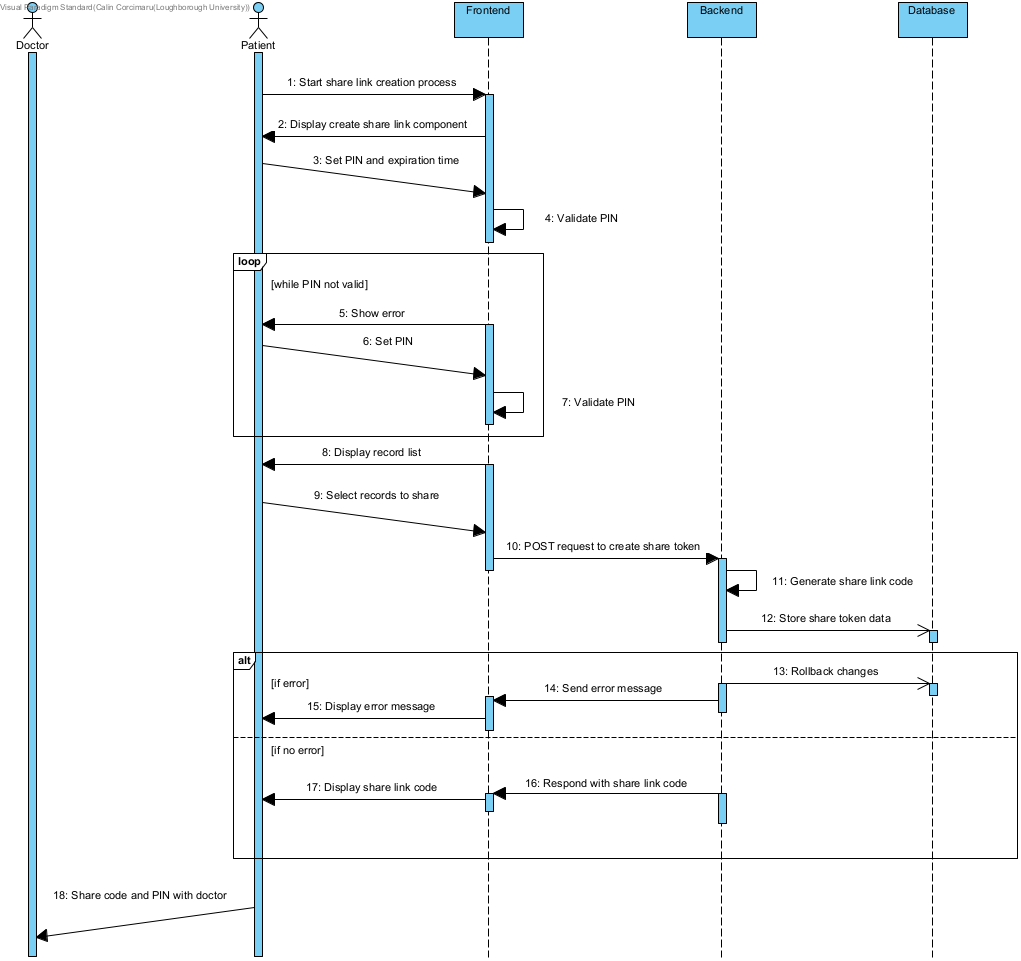
\includegraphics[width=\textwidth,height=0.8\textheight,keepaspectratio]{Sequence_share_updated.png}
  \caption{UML Sequence Diagram --- Creating share link}\label{fig:sequence_share_updated}
\end{figure}

\begin{figure}[htbp]
  \centering
  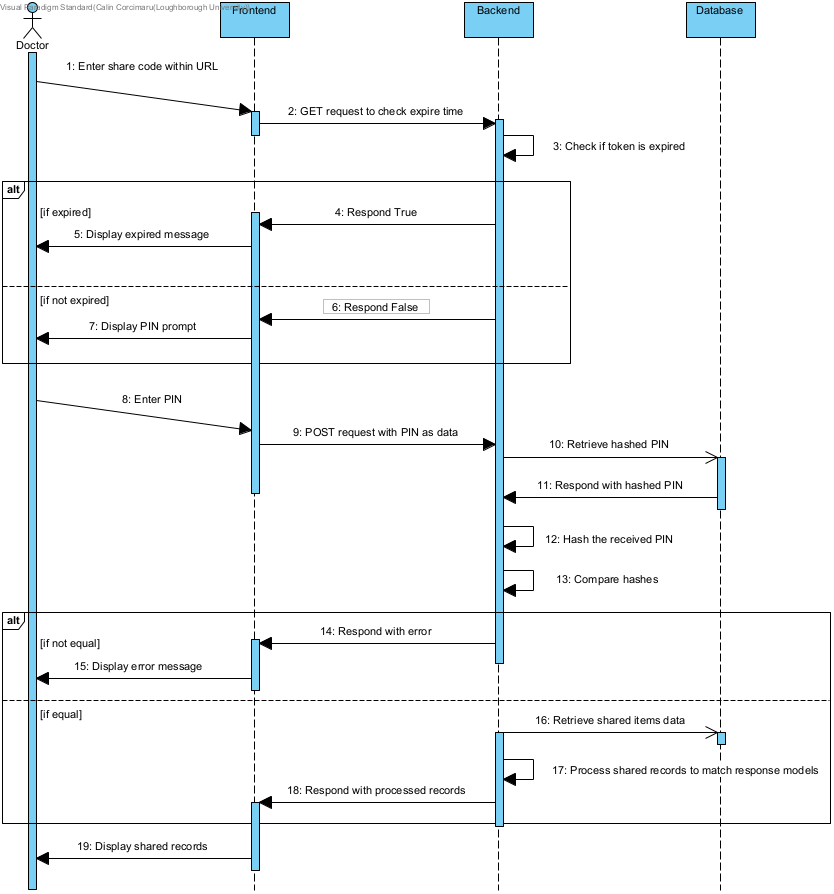
\includegraphics[width=\textwidth,height=0.8\textheight,keepaspectratio]{Sequence_share_access.png}
  \caption{UML Sequence Diagram --- Accessing shared link}\label{fig:sequence_share_access}
\end{figure}

\FloatBarrier{}

\subsection{Frontend changes}

To allow the user to create share links, a new component was created in the frontend. The component was located in the dashboard page, as this is intended to be the main and first page the user sees after logging in. The component was designed to guide the user through the main 3 stages of share link creation: first is the setting of the expiration time and PIN, next is the selection of the records to be shared and finally the confirmation and display of the share link code. The component was designed to be as simple and easy to use as possible, with clear instructions and a step-by-step approach. The component and the different stages can be seen below in figures~\ref{fig:share_create},~\ref{fig:share_records},~and~\ref{fig:share_result}.

\begin{figure}[htbp]
  \centering
  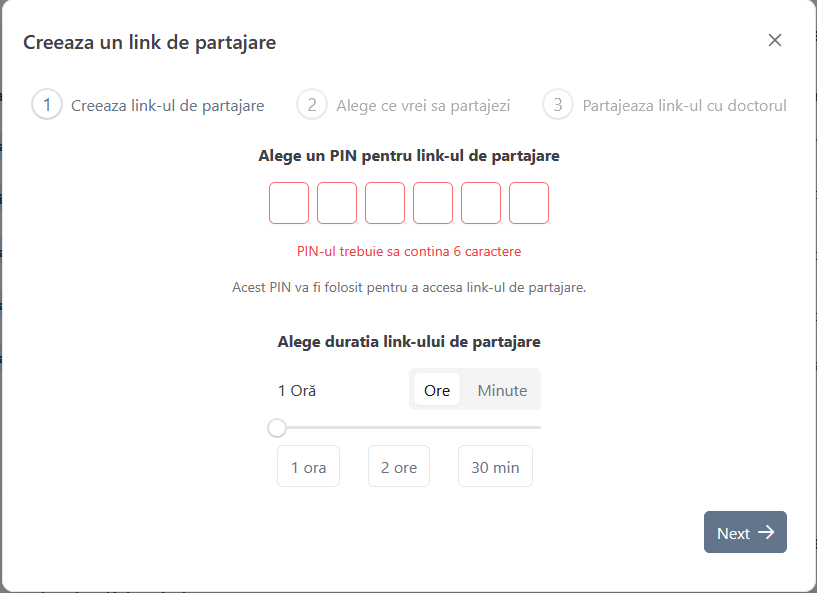
\includegraphics[width=\textwidth]{Desktop_ShareCreate.png}
  \caption{1st step of share link creation}\label{fig:share_create}
\end{figure}

\begin{figure}[htbp]
  \centering
  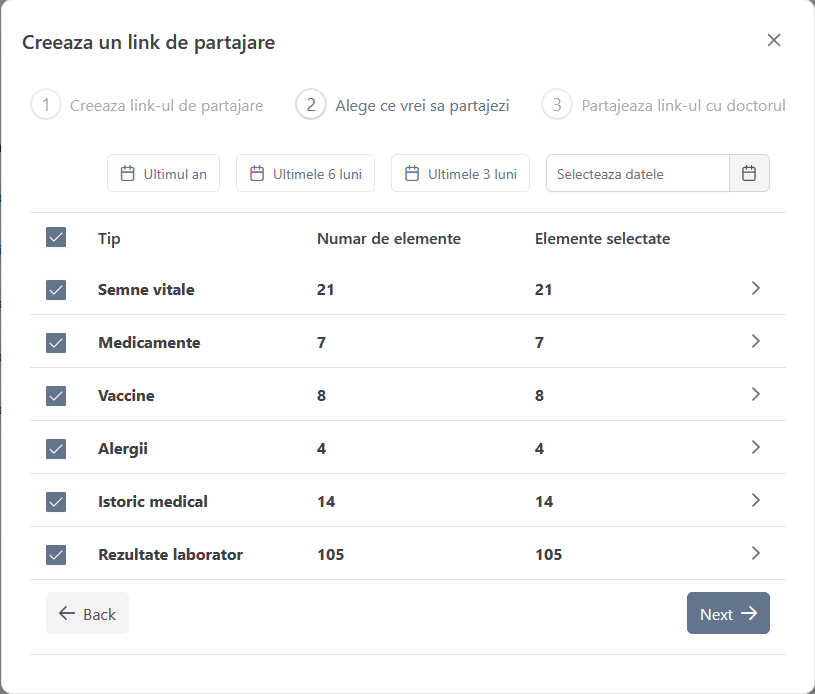
\includegraphics[width=\textwidth]{Desktop_ShareRecords.png}
  \caption{2nd step of share link creation}\label{fig:share_records}
\end{figure}

\begin{figure}[htbp]
  \centering
  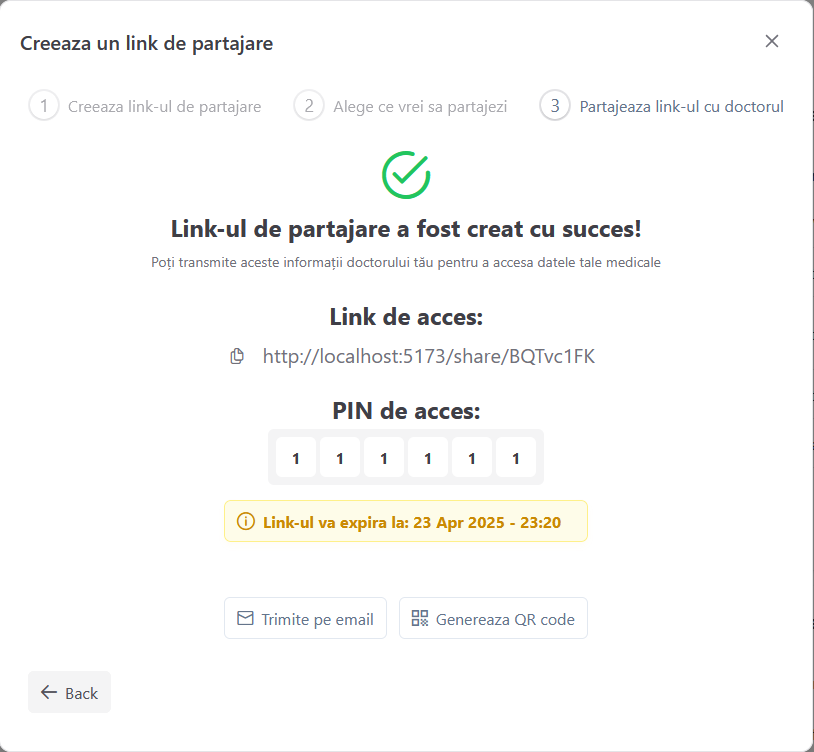
\includegraphics[width=\textwidth]{Desktop_ShareResult.png}
  \caption{3rd step of share link creation}\label{fig:share_result}
\end{figure}

\FloatBarrier{}

Next, the actual page that would display the shared information was created. As described in the previous section, the system would first check the expiration time of the share link, and if valid, would prompt the user to enter the PIN code. If the link would not be valid, the user would be shown an error message and offered the option to be redirected to the landing page. Both of these outcomes can be seen in figures~\ref{fig:share_invalid} and~\ref{fig:share_valid}.

\begin{figure}[htbp]
  \centering
  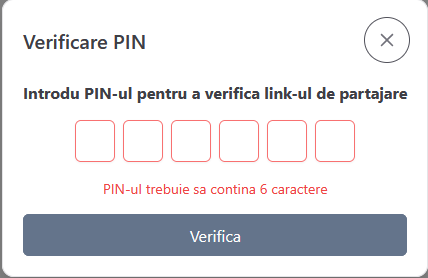
\includegraphics[width=\textwidth]{Desktop_ShareValid.png}
  \caption{PIN prompt dialog}\label{fig:share_valid}
\end{figure}

\begin{figure}[htbp]
  \centering
  
\includegraphics[width=\textwidth]{Desktop_ShareInvalid.png}
  \caption{Expired link dialog}\label{fig:share_invalid}
\end{figure}

\FloatBarrier{}

Finally, to wrap this feature up, the page that would display the shared information was created. Due to the amount of information that could be displayed, it was clear that the previously used tables would not suffice for this task. Since most of the information was displayed in the main system on their own, separate pages, it was important to somehow emulate the same experience without re-creating the pages again. 

This is where PrimeVue's TabView component came in handy, as it added in tabs that allowed the user to switch between the different sections (or record categories), while remaining on the same page. This way, each tab could still contain the table with the records, while having the whole page to display them. The tabs and table columns were dynamically created based on the data received from the backend, in case some of the records were omitted by the user.

Additionally, the page would also contain some basic user information such as the name and date of birth, with potential to add more if the user model would be expanded to contain more information. Finally, a live timer was added to the top of the page to show the time remaining until the link would expire, allowing users to understand how much time they have left to access the information. An example of how the page looks can be seen below in figure~\ref{fig:share_page}.

\begin{figure}[htbp]
  \centering
  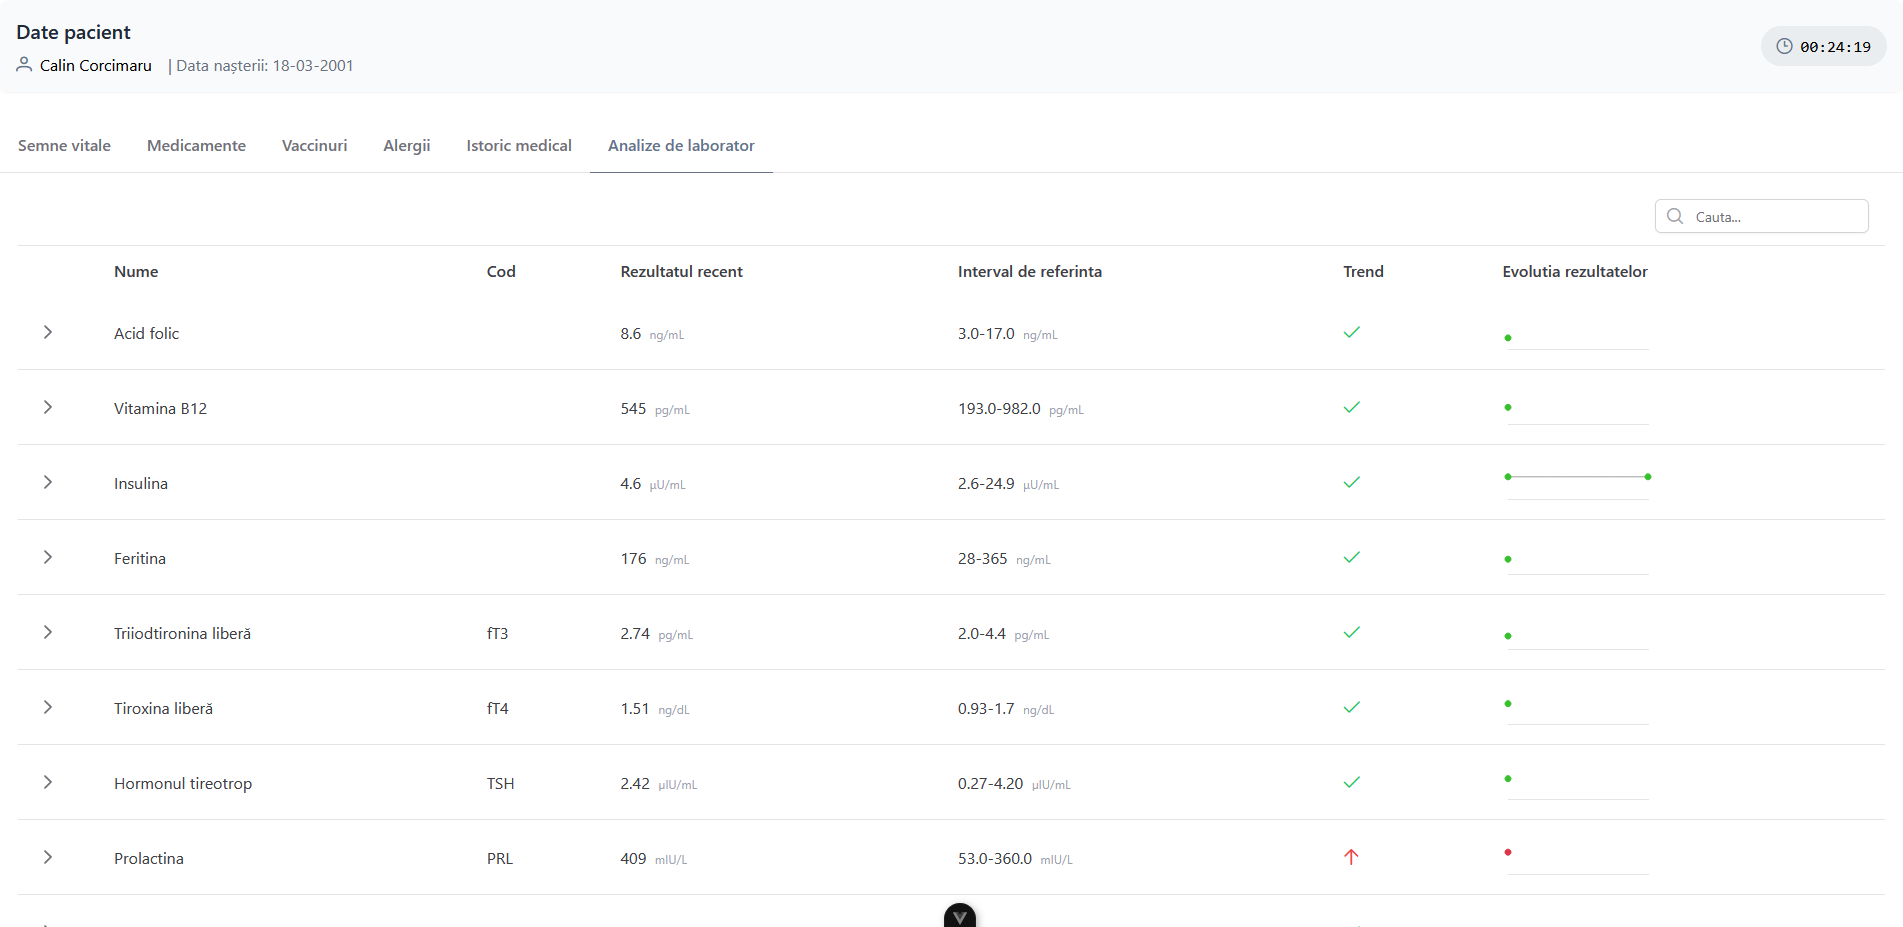
\includegraphics[width=\textwidth]{Desktop_ShareView.png}
  \caption{Share page --- Desktop version}\label{fig:share_page}
\end{figure}

\FloatBarrier{}

\subsection{Backend}

All the backend changes in this sprint were related to the share link feature. A new model was created for the share tokens, which contains the hashed PIN, share code, expiration time and the actual shared items. 

One of the challenges encountered when creating the share token model was the way to store the shared items. The initial idea was to create a new table, which would contain the share item type and their UUID.\@However, this would've added a lot of computation that needed to be done in the backend when creating the share link, as the database would need need to be queried for all items and then they would've have to be processed into their respective response models for the API.\@This would've added unncessary complexity to the system, making it less efficient and harder to maintain if new types of records would be added in the future.

A solution to this problem was to use JSON fields in the database to store the shared items. One of the main reasons for using this method is the origin of the records when choosing them to be shared. Since the share creation link dialog was located in the dashboard, it used the same API response from the dashboard view, which meant that the records were already properly formatted in their respective response models. By using these pre-processed records, a whole step of processing could be avoided: records would be pulled from the dashboard API response, chosen in the share link creation dialog and then stored in the database as a big JSON object as-is. Thus, when accessing the share link, the records would be pulled from the database as a whole JSON object, some light processing done and then directly displayed in the frontend. Additionally, this would reduce the number of queries done to the database, as the items were stored in the same table as the other share token information, such as PIN, share code, etc. 

The updated ERD can be seen in figure~\ref{fig:erd_s6}, making it the last update to the database schema for this project.

\noindent\begin{minipage}{\textwidth}
  \begin{center}
      \rotatebox[origin=c]{270}{
          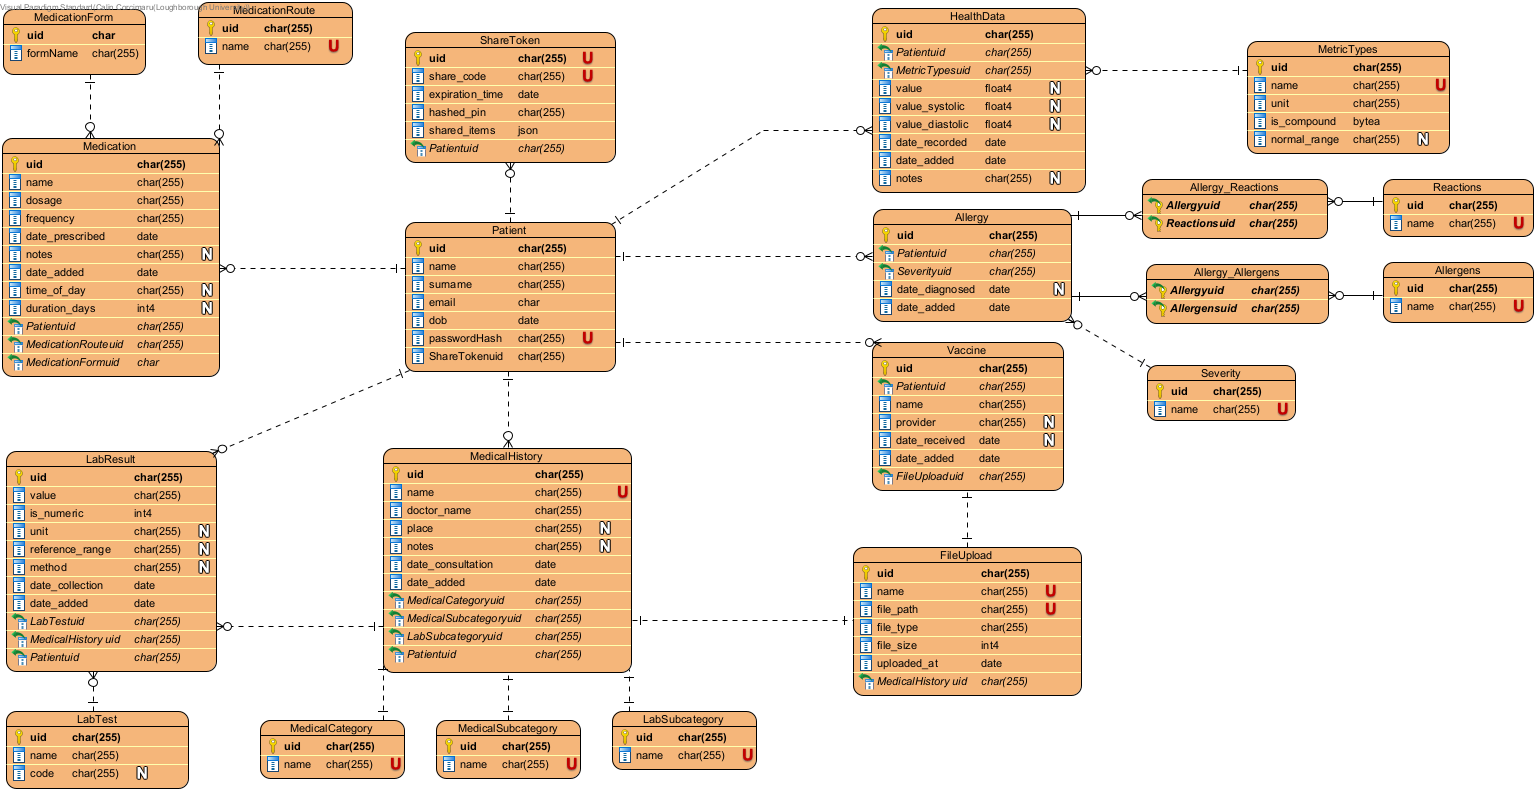
\includegraphics[width=0.95\textheight,keepaspectratio]{ERD_updatedS6.png}
      }
      \captionof{figure}{Updated Entity Relationship Diagram \- Sprint \#6}\label{fig:erd_s6}
  \end{center}
\end{minipage}

\subsection{Challenges encountered}

The main challenge encountered in this sprint was the time pressure, as the project was nearing its deadline. This resulted in some of the features being simplified to their main functionality, without any room for much improvement or additional changes. This was especially true for the frontend part of displaying the shared information, as the amount of data and the combination of the previously added features made it hard to display everything in a single page.

Another interesting challenged encountered was the differences caused by the languages used in the system. As this was a project for patients in Moldova, the frontend was developed in Romanian to accommodate the national language. However most of the code, including the database fields and other models, were written in English as the project was done as part of a degree in a UK-based university. This resulted in some interesting outcomes when data was received from the backend, with many headers being in English, while the rest of the data was in Romanian. In the previously  developed pages, it was possible to manually rename the headers to Romanian, but in the case of the share link items it was very difficult as many of the headers were dynamically created based on the data received. Considering this system was just a prototype, it was deemed acceptable, however for a production system, this issue would've had to be addressed.

\subsection{Requirements completed}

\begin{itemize}
  \item The system must allow the patient to generate a shareable link to provide access to their medical records.
  \item When creating the shareable link, the system must allow the patient to set an expiration date for the link.
  \item When creating the shareable link, the system should allow the patient to set an access password for the link.
  \item When creating the shareable link, the system should allow the patient to select which records to share with the doctor.
\end{itemize}